\documentclass[utf8]{article}
\usepackage{import}
\usepackage{WritingToolsByAcer}

\excludeversion{WritingMaterials}
\excludeversion{backup}


%% ================================== acronym ================================= %
\usepackage{acronym}
\newacro{ntic}[NTIC]{non-trivial informational closure}
\newacro{ic}{informational closure}
\newacro{cg}{coarse-grain}
\newacro{cging}{coarse-graining}
\newacro{cged}{coarse-grained}
\newacro{ncg}{neural coarse-graining}
\newacro{OurTheory}[NCGTC]{The Neural Coarse-graining Theory of Consciousness}


% ============================================================================ %
%                                     Title                                    %
% ============================================================================ %
\title{A neural coarse graining theory of consciousness/\newline Non-trivial Informational closure through neural coarse-graining as the Fundamental Informational Correlates of Consciousness }



% ============================================================================ %
%                                    Authors                                   %
% ============================================================================ %
\author[]{Acer Y.C. Chang\thanks{acercyc@araya.org}}
\author[]{Martin Biehl\thanks{martin@araya.org}}
\author[]{Yen Yu\thanks{yen.yu@araya.org}}
\author[]{Ryota Kanai\thanks{kanair@araya.org }}
\affil[]{ARAYA, Inc., Tokyo, Japan}



% ============================================================================ %
%                                     Body                                     %
% ============================================================================ %
\begin{document}
	\maketitle
	\tableofcontents


	\begin{abstract}
		Neural systems process information through different levels of organisation in a hierarchical manner. Information at lower levels is finer-grained and can be coarse-grained for higher level computation. However, one is aware of information processed only at specific levels. Theorists have addressed this issue. For example, the intermediate level theory of consciousness suggests that the intermediate level seems to be privileged with respect to consciousness. It is true that we do not experience information processed by individual neurons which is always highly noisy. In addition, we have no conscious experience from interpersonal activities despite massive interactions among individuals. Instead, neurophysiological evidence has been showing that conscious experience tends to co-vary with information encoded in coarse-grained neural states such as neural population codes. We argue that the content of consciousness is determined by neural variables that obey informational closure and that other brain processes remain unconscious. Out theory provides a quantitative distinction between conscious and unconscious processing. 
		% Sorry the last part should have been deleted
	\end{abstract}


	\section*{Keywords:}
	Keywords: theory of consciousness, informational closure, neural coarse-graining, level of analysis

    \newpage
    \section*{Not decided terminology}
        \begin{ants}
            @ information * in the NTIC process
            @ Full and short name of this theory
            @ core "?" (entity) for conscious content 
            @ our theory? framework? proposal? 
            @ system? process?
            @ variable? node? element? member?
            @ TODO:
                @@ Change coarse-graining function to "aggregation function"
            @ Decided
                @@ "form" NTIC
        \end{ants}
    

	% ============================================================================ %
	%                                     Start                                    %
	% ============================================================================ %

    \newpage
	\section{Introduction}

		%% Story about a cell
		Imagine you are a neuron in Alice's brain. Your daily work is to collect neurotransmitters through dendrites from other neurons, accumulate membrane potential, and finally send signals to other neurons through action potentials along axons. However, you have no idea that you are one of neurons in Alice's supplementary motor area and involved in many motor control processes for Alice's action, for example, grabbing a cup. You are ignorant of intentions, goals, and motor plans that Alice has at every moment even though you are part of the physiological substrate responsible for all those actions.
		A similar story also happens to Alice's conscious mind. To grab a cup, for example, Alice is conscious of her intention and visuosensory experience of this action. However, her conscious experience does not reflect the dynamic of your membrane potential or the action potentials you send to other neurons every second. That is, information in Alice's conscious experience does not contain information involved in your information processing.

		\toWrite{maybe need a transition sentence here}

		%% scale
		It seems to be true that we are unable to consciously access information processed at every scale in the neural system. Only information at certain levels of coarse-graining can become conscious contents. At microscopic levels of neural systems, information processing in individual neurons is noisy and state transitions of neurons are stochastic \citep{Goldwyn2011, White2000}. However, instead of stochastic action potentials and fluctuation of random noise at microscopic levels, what we are aware of in our conscious mind shows astonishing stability and robustness against the ubiquitous noise in the neural system \citep{mathis1995computational}. Alongside, some parts of the neural system contribute very little to conscious experience (the cerebellum for example \citep{lemon2010life}), also suggesting that conscious contents do not have one-to-one mapping to all parts of the brains. Likewise, experience does not associate with states of the macroscopic brain level because state space of conscious experience is much larger than what a single coarse-grained variable can represent. Additionally, we do not experience "super-consciousness" when we have massive inter-individual interactions with other human-beings. Even though evidence has shown several types of collective information processed at human social groups levels exist \citep{malone2015handbook}, information processed at this level seems to depart from our individual conscious contents.
        \idea{I still think this social example is fine. But the question will become what do we care about? Physical scale or coarse-graining? They are defined in different ways.}


		%% our argument
		In this article, we propose a new theory of consciousness, called \ac{OurTheory}. This proposal states that consciousness does not rest on particular neural architectures or locations in the neural systems. Instead, we argue that consciousness correlates with information processing at a certain coarse-grained level where the neural systems create a high degree of non-trivial informational closure (NTIC)\footnote{In the following NTIC stands for "non-trivial informational closure" or "non-trivially informationally closed".}. We further postulate that the \textit{level} of consciousness corresponds to the degree of NTIC and the \textit{contents} of consciousness corresponds to the state of the NTIC process (for the level versus content of consciousness see \cite{laureys2005neural, overgaard2010neural}).
		
		
		% information-based claim 
		\ac{OurTheory} takes a strong position that consciousness is an information-based phenomenon. I.e. the current proposal can be considered as an information correlate of consciousness (ICC). Based on the presumption, we construct our theory with two core concepts: non-trivial informational closure and neural coarse-graining. In this article, we first introduce non-trivial informational closure and its importance to information processing for human scale agents. We next argue that through coarse-graining the neural system can achieve high degree of non-trivial informational closure at a specific coarse-grained level. We then propose that the state of the informationally closed process correlates with the state of consciousness for both levels and contents which can be explained, quantified, and predicted computationally by our theory. We also illustrate how \ac{OurTheory} can parsimoniously explain empirical findings from previous consciousness studies and reconcile several current major theories of consciousness. Finally, we discuss the current theoretical and empirical limitations of \ac{OurTheory} and propose the implications from this theory to the current consciousness science. 


		\begin{figure}[H]
		    \centering
			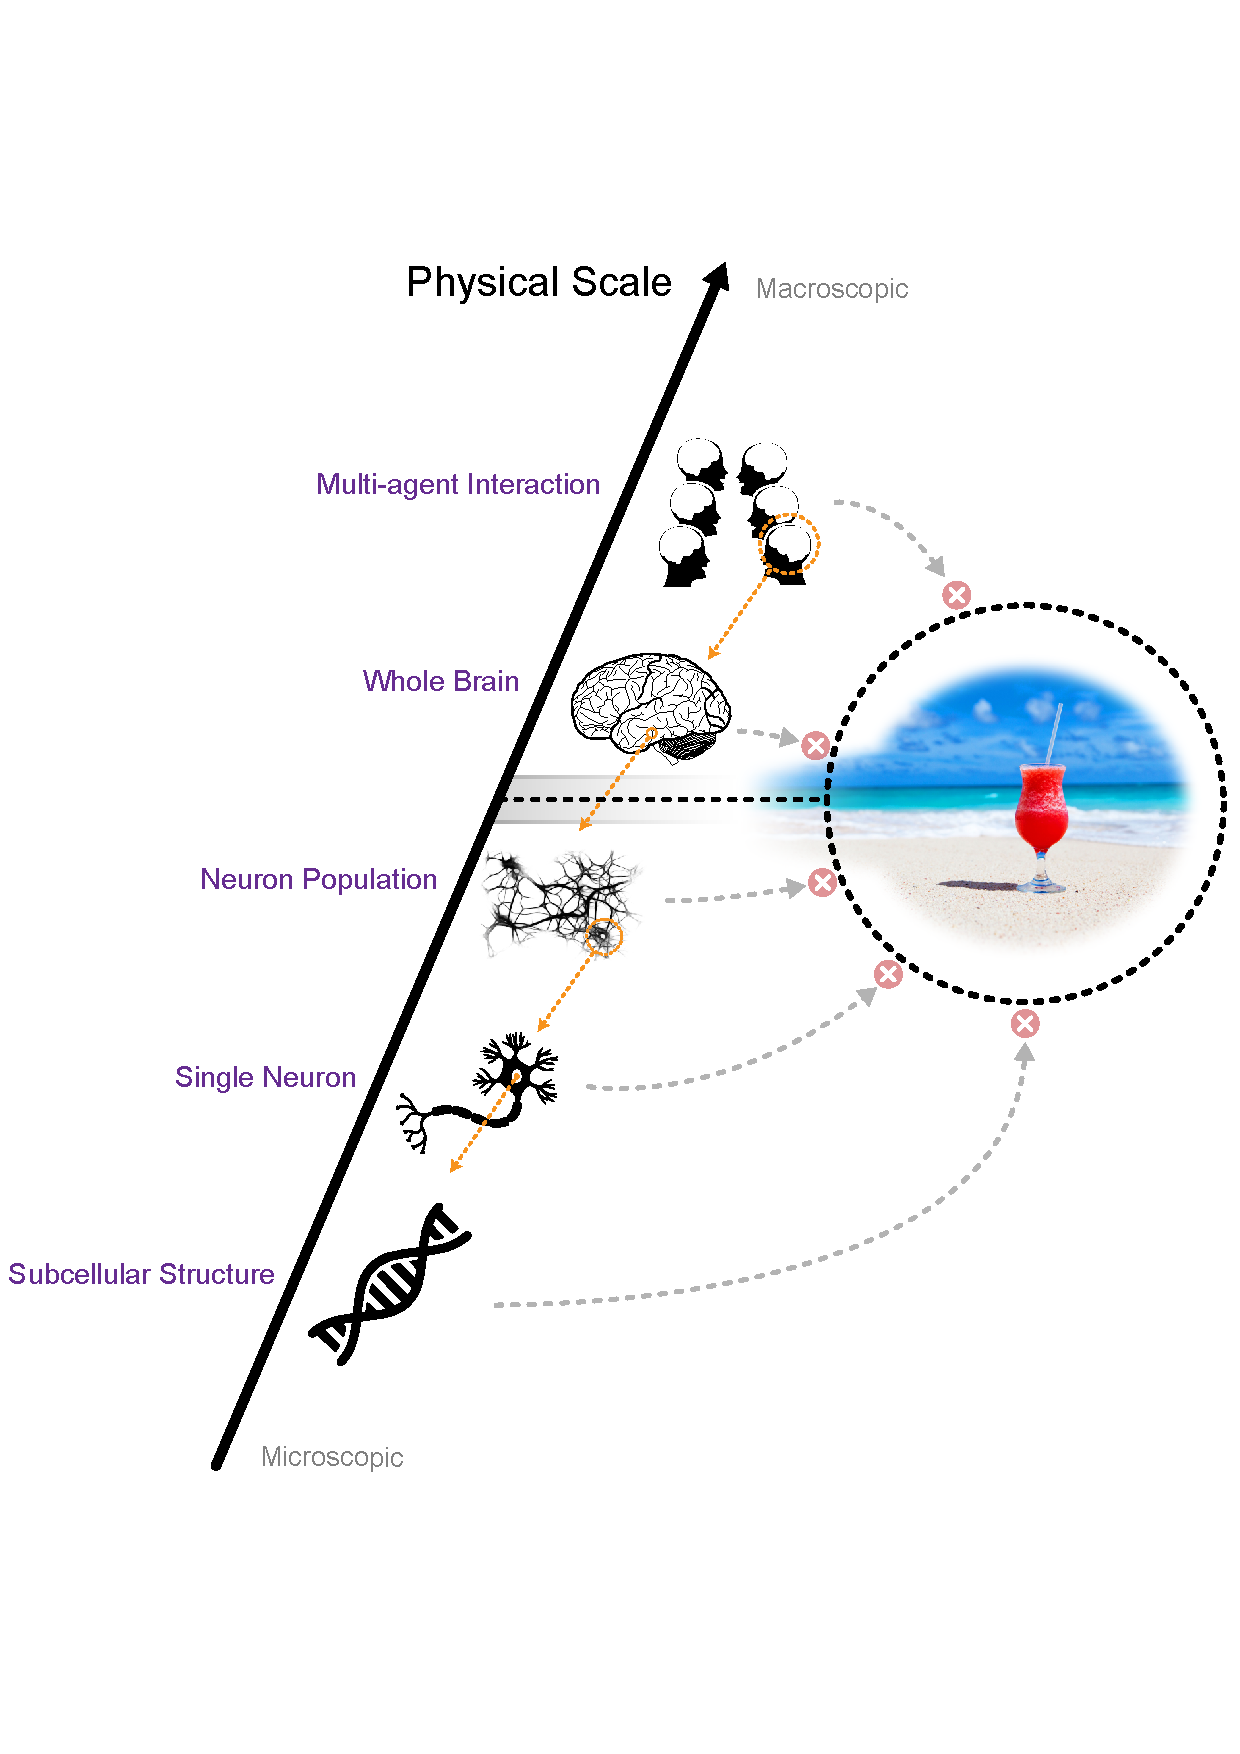
\includegraphics[width=\textwidth]{WritingMaterials/Fig_ScaleProblemOfConsciousness/ScaleProblemOfConsciousness.pdf}
			\caption{The scale problem of consciousness}
	   	\end{figure}



		%% backup point
		\begin{WritingMaterials}
			@ consciousness is information

			@ conscious contents
				@@ \toWrite{lower level}
				@@ Information processing of individual neurons are noisy.
				@@ We don't have conscious content changes when individual neurons fire action potentials.
				@@ Don't even mention ion channel dynamic.


				@@ \toWrite{Higher-level dynamic}


			@ For human, physics at our body scale are nearly follow classic physics, which is deterministic.


			@ \toWrite{Human tendency for active prediction }
				@@ \cite{Stahl2015} \rewrite{
					Given the overwhelming quantity of information available from the environment, how do young learners know what to learn about and what to ignore? We found that 11-month-old infants (N = 110) used violations of prior expectations as special opportunities for learning. The infants were shown events that violated expectations about object behavior or events that were nearly identical but did not violate expectations. The sight of an object that violated expectations enhanced learning and promoted information-seeking behaviors; specifically, infants learned more effectively about objects that committed violations, explored those objects more, and engaged in hypothesis-testing behaviors that reflected the particular kind of violation seen. Thus, early in life, expectancy violations offer a wedge into the problem of what to learn.}

			@ Intuitive physics \needref{Intuitive physics}

		\end{WritingMaterials}






	\section{Non-trivial informational closure} \label{sec:Non-trivial informational closure}
		The notion of non-trivial informational closure (NTIC) is introduced by \cite{BERTSCHINGER.2006}. The concept of closure is closely related to system identification in systems theory. One can distinguish a system from its environment by computing the closedness of the system \citep{maturana1991autopoiesis, rosen1991life, pattee2012evolving, luhmann1995probleme}. The closedness can be further quantified by information theory.

		\begin{WritingMaterials}
			@ Consciousness as an intrinsic information. Therefore, information should be self-define. This means the boundary of conscious content should be related to informational closure.

			@ \idea{should we describe the intuition of boundary problem here?}

			@ ============================================================================


			@ \rewrite{
				The notion of closure plays a prominent role in systems theory where it is used to identify or define the system in distinction from its environment} \cite{BERTSCHINGER.2006}

			@ \rewrite{
				Our theoretical interest concerns the type of system that is a unity for and by itself and not only for an external observer distinguishing some entity from the rest of the world. This requires a system that can be described as a whole without reference to its environment. In systems theory, this property is usually referred to as closure.}\citep{BERTSCHINGER.2006}

			@ \rewrite{
				These concepts of closure play an important role in the architecture of systems
				theory, because they are used to
				1. define the system (in distinction to its environment) and to
				2. explain the autonomy of the system.}\citep{BERTSCHINGER.2006}

			@ \rewrite{
				Informational closure: The higher process is informationally closed, i.e., there is no information flow from the lower to the higher level. Knowledge of the microstate will not improve predictions of the macrostate.} \citep[p. 4]{PFANTE.2014}


		\end{WritingMaterials}


		% Definition of informational closure
			\noindent
			Consider two processes, the environment process $(E_t)_{t \in \mathbb{N}}$ and the system's process $(Y_t)_{t \in \mathbb{N}}$ and let their interaction be described by the Bayesian network in Figure~\ref{fig:SystemAndEnv}. Then, information flow $J_{t}$ from the environment $E$ to a system $Y$ at time $t$ can be defined as the conditional mutual information $I$ between the current environment state $E_{t}$  and the future system state $Y_{t+1}$ given the current system state $Y_{t}$

				\begin{equation}
    				\label{eq:InformationFlow}
    				\left.\begin{array}
    				{rl}{J_{t}(E \rightarrow Y )} & {:= I(Y_{t+1};E_{t}|Y_{t})} \\
    				%{ } & { \ = H(Y_{t+1}|Y_{t})-H(Y_{t+1}|Y_{t},E_{t})} \\
    				%{ } & { \ = H(E_{t}|Y_{t})-H(Y_{t}|Y_{t},Y_{t+1})} \\
    				%{ } & { \ = H(E_{t}|Y_{t})-H(E_{t}|Y_{t},Y_{t+1})}\\
    				{ } & { \ = I(Y_{t+1};E_{t}) - (I(Y_{t+1};Y_{t})-I(Y_{t+1};Y_{t}|E_{t}))}
    				\end{array}\right.
				\end{equation}

				\begin{figure}
					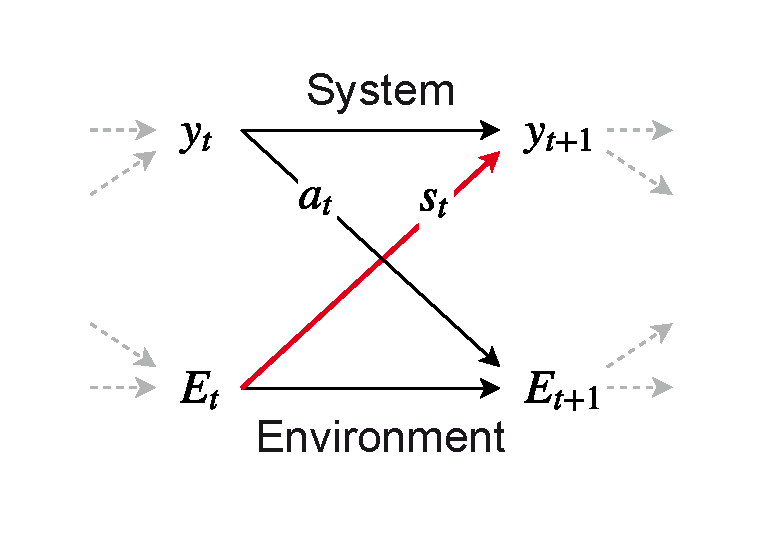
\includegraphics[width=\textwidth]{WritingMaterials/Fig_SystemAndEnv/SystemAndEnv.pdf}
					\caption{Figure adapted from \cite{BERTSCHINGER.2006}}
					\label{fig:SystemAndEnv}
				\end{figure}


			\noindent
			\cite{BERTSCHINGER.2006} defines that a system is informationally closed when information flow from the environment to the system is close to zero.

				\begin{equation}
				J_{t}(E \rightarrow Y )=0
				\end{equation}


			% ------------------------------- trivial case ------------------------------- %
			\noindent
			Information closure (minimising $J_t$) is trivial if the environment and the system are entirely independent of each other.

				\begin{equation}
				\begin{aligned}
				{I(Y_{t+1};E_{t})=0}&&{\Rightarrow}&&{J_{t}(E \rightarrow Y )=0}
				\end{aligned}
				\end{equation}


			% -------------------------------- non-trivial ------------------------------- %
			\noindent
			However, informational closure can be achieved non-trivially. In the non-trivial case, even a system that contains (or encodes) information about the environment is still informationally closed. This means

				\begin{equation}
				I(Y_{t+1};E_{t}) > 0
				\end{equation}

			\noindent
			This also implies
				\begin{equation}
					I(Y_{t+1};Y_{t})-I(Y_{t+1};Y_{t}|E_{t}) > 0
				\end{equation}



			\noindent
			And, non-trivial informational closure can be defined as
				\begin{equation}
				\label{eq:NTIC}
    				\left.\begin{array}
    				{rl}{NTIC} & {:=I(Y_{t+1};Y_{t})-I(Y_{t+1};Y_{t}|E_{t})}
    				\end{array} \right.
				\end{equation}
				
				
			\noindent
            The definition can also be re-arranged as 
				\begin{equation}
				\label{eq:NTIC2}
    				\left.\begin{array}
    				{rl}{\qquad} & {\ =I(Y_{t+1};E_{t})-I(Y_{t+1};E_{t}|Y_{t})}
    				\end{array} \right.
				\end{equation}				

			\noindent
			Hence, maximising NTIC amounts to
				\begin{equation}
    				\label{eq:nticObjective}
    				\begin{aligned}
    				& \text{maximising} & { } & I(Y_{t+1};Y_{t}) & { } & \text{and} \\
    				& \text{minimising} & { } & I(Y_{t+1};Y_{t}|E_{t}) & { }
    				\end{aligned}
				\end{equation}

			\noindent
			This implies the system contains in itself all the information about its own future and the self-predictive information is gained from the information about the environment. Therefore, to achieve NTIC, the system can internalise and synchronise the dynamics of the environment, i.e. modelling the environment. Furthermore, having high degrees of NTIC entails having high predictive power about the environment. This gives biological agents a great functional and evolutionary advantage. Practically, \cite{guttenberg2016neural} proposed that NTIC can be achieved by maximising the predictive power about the environment and the self-predictive information of the system concurrently.


			% Biological evidence of informational closure in the neural system
			Despite the significant advantage for biological systems to achieve NTIC, to our knowledge, studies directly examining NTIC in biological systems are limited. However,  recent studies have shown relevant properties in the visual system of salamanders. By examining the salamander retina, in two studies \citep{Palmer2015, sederberg2018learning} the authors found that the a large groups of neural populations of retinal ganglion cells encoded predictive information about external stimuli also had high self-predictive information about their own future states (see Figure~\ref{fig:sederberg2018learning}), therefore, in line with the characteristic of NTIC. Therefore, the self-predictive information of the neural populations can guide prediction about external stimuli without reference to stimulus parameters explicitly. Moreover, the internal predictability can be generalised to different stimulus classes suggesting the tendency to internalise the information of environmental dynamics in the neural populations. \toWrite{Add Some ending sentences}


			\begin{figure}[H]
				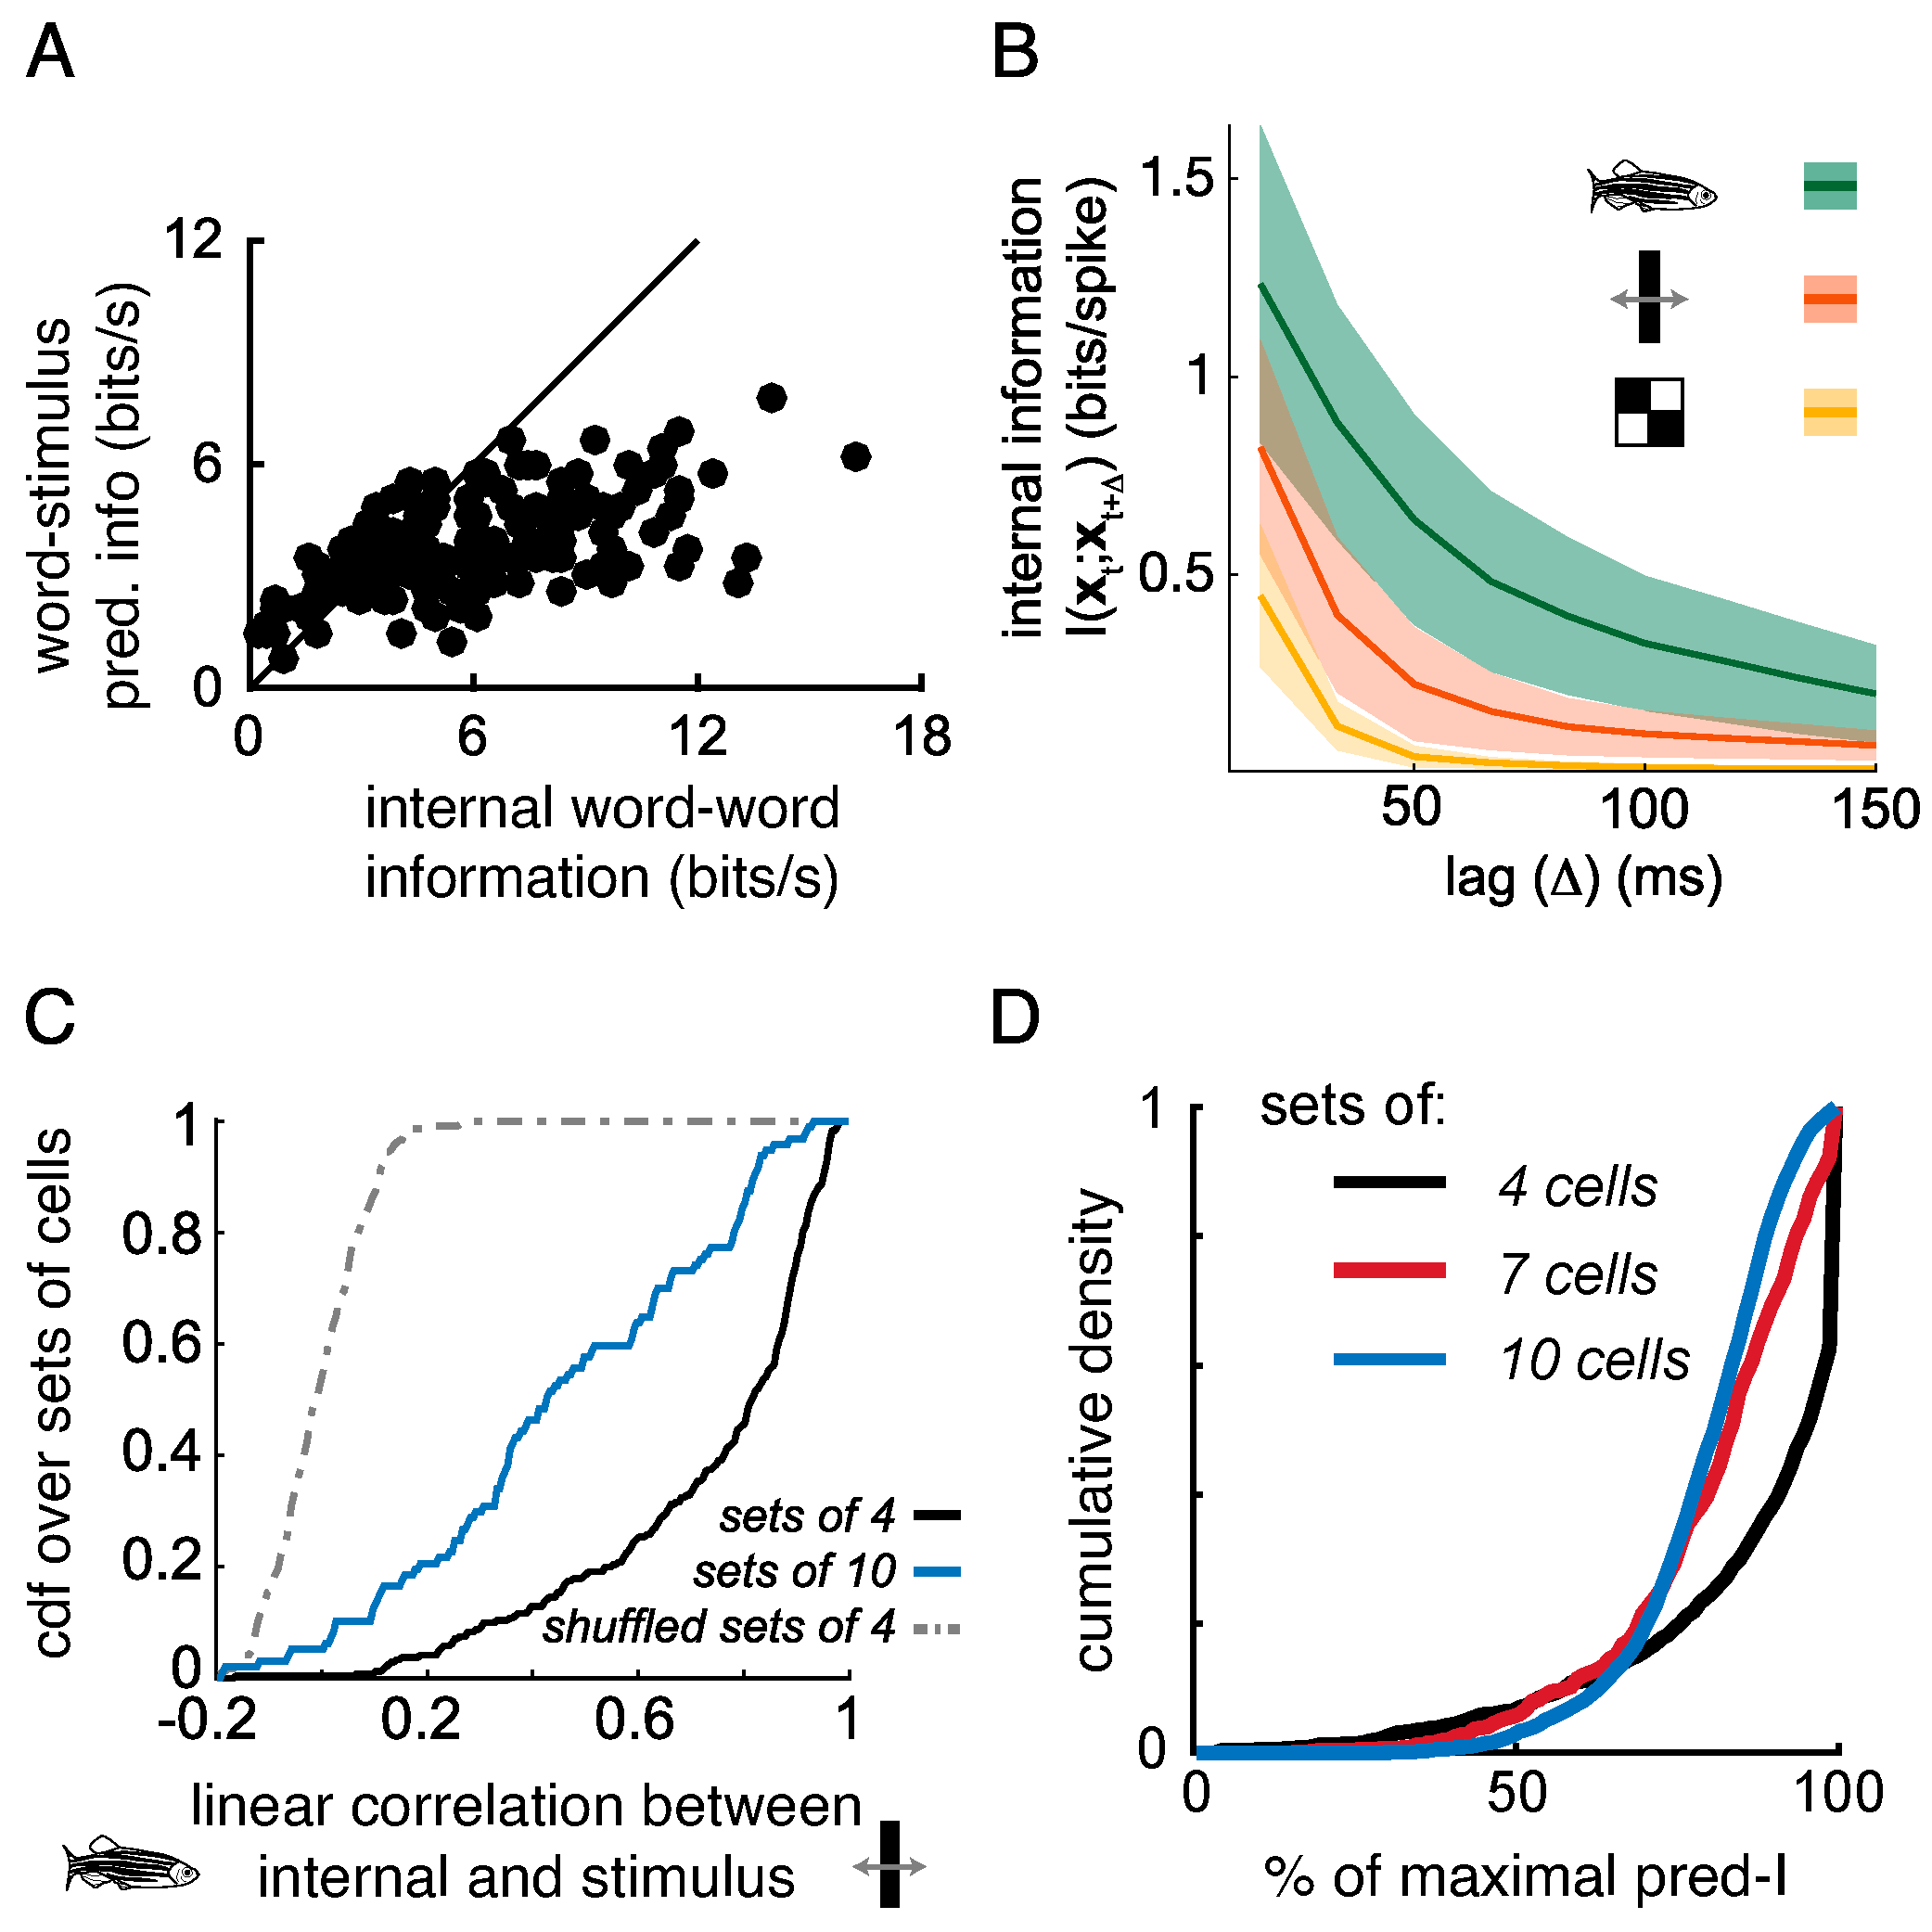
\includegraphics[width=\textwidth]{WritingMaterials/Fig_Sederberg/Fig_Sederberg.pdf}
				\caption{Figure adapted from \cite{sederberg2018learning}}
				\label{fig:sederberg2018learning}
			\end{figure}

			\begin{comment}
				@ ===

				@ \rewrite{
					Internal information reflects the spatial and temporal correlations in the stimulus.}

				@ \rewrite{predictive information is encoded synergistically.}

				@ \rewrite{
					in recordings of populations of RGCs of salamander retina driven by a simple stimulus with partially predictable dynamics, joint activity patterns transmit information that is predictive of future stimuli }

				@ \rewrite{
					We examined whether the temporal correlations within populations of RGCs can be used to guide the search for readouts of predictive information.}

				@ \rewrite{
					We showed that groups of cells with high external, stimulus-predictive information also had high internal predictive information on two classes of stimuli, }

				@ \rewrite{
					Very simple learning rules could find near-optimal readouts of predictive information without any external instructive signal. This suggests that bottom-up prediction may play an important role in sensory processing}

				@ \rewrite{
					Internal predictive information can guide stimulus prediction without explicit reference to stimulus parameters.}

				@ \rewrite{
					Word–word internal predictive information is correlated with word–stimulus predictive information across sets of four cells.}

				@ They also showed generalization of internal predictability across stimulus. This suggests .... what?

				@ \rewrite{
					The generalization of internal predictability across stimulus classes partially reflects the ability of the retina to adapt to the statistics of stimuli}


				@ \cite{Palmer2015}
				@ \rewrite{
					Groups of cells in the retina carry information about the future state of their own activity, and we show that this information can be compressed further and encoded by downstream predictor neurons that exhibit feature selectivity that would support predictive computations.}

				@ \rewrite{
					It seems natural to phrase the problem of prediction in relation to the visual stimulus, as in Fig. 3, but the brain has no direct access to visual stimuli except that provided by the retina. Could the brain learn, in an unsupervised fashion, to predict the future of retinal outputs? More precisely, if we observe that a population of retinal ganglion cells generates the word w t at time t, what can we say about the word that will be generated at time t + delta t in the future? The answer to this question is contained in the conditional distribution of one word on the other, P ð w t +delta t j w t Þ } \url{http://tinyurl.com/y9zmhlln}

				@ \rewrite{
					larger groups of cells carry predictive information for hundreds of milliseconds, }



			\end{comment}



			%% backup
			\begin{comment}
				@ Accurately model deterministic environment
				@ \rewrite{
					This demonstrates that a system exhibiting certain internal regularities as measured by $A^* = MI(Sn+1; Sn)$ can achieve informational closure either by gaining information about the environment or by increased autonomy, i.e. by becoming unpredictable or uncontrollable from the (13) environment. Therefore, information about the environment, i.e. modelling, and autonomy can be considered as complementary strategies for achieving informational closure.}

				@ By Action

				@ In the next section, we claim that the neural system achieve NTIC through coarse-graining.
			\end{comment}
			


	\section{Neural coarse-graining}

		%% stochasticity at microscopic levels
		To create NTIC in a highly stochastic system (e.g., the neural system) is challenging. The more a system is influenced by the environment the more information about the environment's state it has to contain itself. This however requires the predictability of the environment state and is therefore impeded by noisy environments.  Information processing at the microscopic levels (the cellular levels) in the neural system suffers from multiple environmental noise sources throughout, including sensory, cellular, electrical, and synaptic noises. Previous studies have shown that states of neurons have large trial-to-trial variability at the cellular level. That is, the same pattern of activity never occurs twice even when the same stimulus is presented. Neurons are inevitably subject to thermal fluctuations and other physical noises \citep{faisal2008noise}. Furthermore, environmental information is always only partial observable to individual sensors and neurons which only receive little amount of information from the environment. Therefore, information about the environment state at the cellular level is difficult to represent. It is implausible to construct NTIC processes at microscopic levels.

        %% Our argument
        \critical{Need Discussion}
		However, we argue that, neural systems can form NTIC at certain macroscopic levels by coarse-graining microscopic neural states. Despite the microscopic levels in the neural system is stochastic and difficult to form NTIC processes, one solution to overcome the difficulty is to coarse-grain and encode information in coarse-grained variable to form stable and robust representation in the system. Coarse-graining refers to many-to-one functions that map microscopic states to macroscopic states.\needref{Do we need reference?}. In other words, a number of different micro-states realise the same value of the macro-variable \citep{price2007causation}. This is a common neural coding strategy that we can see in large number of previous neurophysiological studies. For example, in the temporal domain, neural spikes across time can be coarse-grained as spiking rate variables, known as rate coding \citep{adrian1926impulses, gerstner2002spiking, maass2001pulsed, panzeri2015neural, stein2005neuronal}. Neurons encode stimulus intensity by increasing or decreasing firing rate. \citep{kandel2000principles}. In this coding scheme, individual neural spikes in a transient time span are not meaningful and stochastic \citep{stein2005neuronal}. In contrast, rate codes are relatively stable and are highly robust against noise caused by the variation of inter-spike intervals. 
		
		% population code
		Another example of coding strategy using coarse-graining is population coding. In this coding scheme, information is represented by joint spatiotemporal activities of several neurons. Therefore, the information is encoded in coarse-grained variables whose values are jointly determined by neural activation patterns within a neural population \citep{kristan1997population, pouget2000information, binder2009encyclopedia, QuianQuiroga2009}. In such cases, activities of every single neuron is not informative and stochastic. Instead, coarse-grained variables (such as population averaging and population vector) are able to represent information more stably. Encoding information at coarse-grained levels allow the neural system to ignore certain causal interactions relevant to fine-grained level of description \citep{Woodward2007-WOOCWA}.
			
			
		% neural coarse-graining by Nic
		As mentioned above, it has been empirically shown that NTIC can be achieved by coarse-graining sensory inputs in artificial neural networks. \citep{guttenberg2016neural} proposed a "neural coarse-graining (NCG)" architecture (fig.\ref{fig:NCG}) which aims to capture the emergent large-scale dynamics in the environment. The NCG network learns to coarse-grain input signals and extract latent parameters which are both predictive and predictable in the input signal and therefore achieves NTIC by building a higher-level representation of the underlying dynamics in the deep layers. More importantly, using this architecture, agents can process information and act at coarse-grained macroscopic levels.
		
		\begin{WritingMaterials}
    		% --- This figure is not necessary now ---
    		\begin{figure}
    			\includegraphicsTodo[width=0.8\textwidth]{WritingMaterials/Fig_temp/PDFXCview_2018-06-08_14-24-03.png}
    			\caption{NCG \idea{I need to simplify this figure}\citep{guttenberg2016neural}}
    			\label{fig:NCG}
    		\end{figure}		
    	\end{WritingMaterials}

		%% not monotonic
		It is important to note that NTIC can be a non-monotonic function of scale of coarse-graining. If macroscopic variable is overly coarse-grained the system states can result in low degrees of NTIC. For example, in an extreme scenario, when all microscopic states map to a single macroscopic variable, the macroscopic level does not have any information capacity and thus looses the self and environmental predictive power. The non-monotonic relationship is also supported by empirical evidence. \cite{sederberg2018learning} showed that the efficiency of reading out self-predictive information of neural population is higher when the number of cells in a populations is 4 than it is when that number is 7 or 10 cells. This implies an optimal coarse-graining scale for NTIC processes. % Perhaps the best way to combine more than four cells is to break down the readout into indivisible units of four cells, which are later recombined in subsequent processing.}\citep{sederberg2018learning}


        %% Link to consciousness
        At the physical scale which human beings live in, the environmental dynamics is nearly deterministic following the laws of classical physics. This suggests that information in the environment is nearly closed at a right spatial-temporal scale. Therefore, this gives agents living at this physical scale great advantages if the agents form a NTIC process internally. Therefore, coarse-graining becomes necessary to map microscopic sensory and neuronal states into macroscopic NTIC process. 
        
        %This means that it is possible for agents to live at this physical scale to build NTIC process internally.
    % More importantly, the information processing related to consciousness should not be situated at this level. Otherwise our conscious percept should be very noisy and unstable.
        



		\begin{WritingMaterials}
			@ \rewrite{
				Coarse-graining: a method of reducing the complexity of a system by treating groups of atoms/molecules as single quasi-particles CG: coarse-grained}

			@ neural system use population coding and temporal coding to fight against noise.

			@ Therefore, even though the low level information processing is noisy, it is possible that the neural system achieve NTIC at a coarse-grained level.

			@ This implies that the information about the environmental dynamic should be represented at a certain coarse-grained level rather then other levels.

			%% Microscopy Deterministic
			@ The environment that human scale agents interact with is approximately govern by Newton's law and therefore the state transitions are nearly deterministic.

			@ \idea{Need something here}
			
			%% coarse-graining is necessary
			@ Hence, to coarse-grain states of microscopic levels is necessary to represent and model the human-scale environment state and dynamics.

			@ Coarse-graining is necessary to resist noise

			@ \rewrite{ The population will therefore be relatively insensitive to the loss of
				cells or noise in a small number of cells} \cite{eurich2000multidimensional}


			@ Studies have shown that coarse-graining is a common way that the neural system cope with inevitable noise at microscopic levels.

			@ \rewrite{Because the sequence of action potentials generated by a given stimulus varies from trial to trial, neuronal responses are typically treated statistically or probabilistically}


			@ Note that, information processing related to consciousness should not be situated at this level. Otherwise our conscious percept should be very noisy and unstable.

			@ Population coding

				@@ review ref

					@@@ \cite{Stanley2013}

					@@@ \cite{QuianQuiroga2009}

				@@ \rewrite{
					Averaging is used in many neural systems in which information is encoded as patterns of activity across a population of neurons that all subserve a similar function (for example, see REFs 140,141 )}
									140. Georgopoulos, A., Schwartz, A. \& Kettner, R. Neuronal population coding of movement direction. Science 233, 1416–1419 (1986). 141. Lee, C., Rohrer, W. H. \& Sparks, D. L. Population coding of saccadic eye movements by neurons in the superior colliculus. Nature 332, 357–360 (1988).

				@@ \rewrite{
					Electrophysiological studies in the monkey have shown that behaviourally relevant signals are averaged not only across neuronal populations but also over time in the formation of a behavioural decision 156 .} 156. Gold, J. I. \& Shadlen, M. N. Representation of a perceptual decision in developing oculomotor commands. Nature 404, 390–394 (2000).


				@@ \rewrite{A distributed representation of information of this type is more robust to the effects of noise.}



				@@ \rewrite{
					Neural population code: the set of response features of a population of neurons that carry all information about the considered stimuli. These features consist of spatial-temporal sequences of action potentials distributed across neurons and/or time.}

				@@ The diverse response selectivity of sensory neurons

				@@ \rewrite{
					How a neural population represents information is partly determined by the diverse selectivity of individual neurons \cite{Shamir2014}}



				@ sensory hierarchy
					@@ sensory hierarchy also shows characteristic of coarse-graining


					@@ Due to partial information that sensors can receive

					@@ To form complex representation like shape, objects, coarse-graining is necessary.


					@@ Through coarse-graining, \highlightAndComment{higher level}{might be confusing, need to think about the terminology here} cortical areas can integrate those partial information to infer hidden causes.

				

				@ Through two objectives during training, the model can achieve NTIC.

				@ this can be achieved by maximising the self-predictive power of deep layers and its entropy through all training data.

				@ With the objectives, NCG network learns to coarse-grain input signals and  extract latent parameters which are both predictive and predictable in the input signal and therefore achieves NTIC by building a higher-level representation of the underlying dynamics in the deep layers.

                @ \ideaBox{Consider the two points}
                @ ----------------------------------------------------------------------------
                @ Achieving NTIC is the key objective to to extract out latent control parameters in the environment.
				@ Agents can process information and act at abstract levels
				@ ----------------------------------------------------------------------------
			    

				@ At the physical scale which human being live, the environmental dynamics is nearly deterministic following the laws of classical physics. This means that it is possible for agents living at this physical scale to build NTIC process internally.

				@ When the information in individual sensory channel is noisy and partial, coarse-graining becomes necessary for achieve NTIC.
			\end{WritingMaterials}




% ============================================================================ %
%               A neural coarse graining theory of consciousness               %
% ============================================================================ %
	\section{A neural coarse graining theory of consciousness}
	


        In this section, we propose a new theoretical framework of consciousness: \acf{OurTheory} \todo{We really need a good name}. The Theory offers two propositions:
        \begin{enumerate}
            \item We argue that the existence of an NTIC process within a system is sufficient for information processing to be conscious.
            \item  For the neural system that achieves NTIC must necessarily satisfy coarse-graining
        \end{enumerate}

        In what follows, we will first establish two presumptions on which this Theory depends. Then, we will develop the propositions in detail. 
        
        The first presumption is that every human conscious precept is highly informative. Here, "informative" refers to the resolution of uncertainty. Being in a certain conscious state rules out an enormous number of other possible conscious states. This is in line with the impression that our conscious experience consist of highly multidimensional information and usually involves information from multiple modalities. Therefore, every conscious precept resolves a huge amount of uncertainty and provides considerable information.  
        
        This presumption is in agreement with one of the axioms, \textit{information}, in Integrated Information Theory (IIT 3.0) which claims that \myQuote{...an experience of pure darkness is what it is by differing, in its particular way, from an immense number of other possible experiences...} \citep[p. 2]{oizumi2014phenomenology}.
        
        Based on this presumption, we postulate that the amount of (self-)information possessed by a conscious percept should be equal to the (self-)information of a particular event or entity in the physical reality. In this theory, we consider information is the common language between conscious experience and the physical reality. We further take a radical standpoint and postulate that consciousness is fundamentally associated with specific kind of information, i.e., the information correlates of consciousness (ICC), \cite{chalmers1996conscious, tononi2004information, gamez2011information, Gamez2016}) and discard the notion of neural correlates of consciousness(NCC). 
        
        The second presumption is that the amount of information in consciousness is bounded. Even though information involved in every conscious percept is extremely rich, it is still limited and we do not consciously feel everything in this universe. This leads to the boundary problems of consciousness \cite{goff2006experiences}. There should exist information boundaries for every conscious entity. If consciousness is an information-based phenomenon, we should be able to identify the boundaries with measures of information theory. Specifically, we claim here that boundaries are defined by information closure. Therefore, information closure should be observed in physical systems with consciousness . 
        
        
        \rewording{informational closure also suggests that there is no information flow from the lower to the higher level. Knowledge of the microscopic levels will not improve predictions of the future states of the macroscopic levels \citep{PFANTE.2014}}. 
        Information closure also implies that the system is ignorant of information outside of the system. Therefore, if a coarse-grained level achieves information closure, it suggests the NTIC process at the coarse-grained level is ignorant of information processing happening at microscopic levels and also higher coarse-grained levels. This virtually makes the informational closed macroscopic levels as a complete reality. 
        \todo{Due to my concern mentioned last week, I think I should also mention the closure is not only to the environment but also to the microscopic levels}
        
        Finally, our conscious experience always reflects some information about environment and bodily states, i.e. non-trivial information. To account for the information-based considerations, we propose that NTIC is a fundamental informational property associated with consciousness. 
        
        \ideaBox{Informational closure and level identification}
        
        
        \begin{WritingMaterials}
        For example, considering two physical systems (Alice and Bob) and there is no interaction (or information passing) in between. Assuming that Alice is conscious, the conscious experience that Alice has should not involve any information about Bob. 
        
        \todo{Considering putting this para}
        Similarly, we can apply this scenario to brain processing between two regions. We can consider a thought experiment. 
        Imagining that in the future, one poor subject attend this experiment. We remove the subject's visual cortex from other brain areas. However, we keep all the connection between the two parts of the brain intact by replacing dendrites and axons between the two parts with micro electronic cables. Because these cables are very long, we can move the visual cortex to the surface of Mars. Now the experimenters give visual cortex a input signal. If the signal travels with the speed of light, it still takes three seconds to reach the other part on the earth. We can ask: Between the experimenters send the input signal and the information reach the part on the earth, what visual conscious content does the subject experience in the three seconds? We presume that in this three seconds subject's conscious experience should not contain any information about the visual input. Otherwise, the subject may be able to use the information to perform subsequent actions. This violates physics. This may look like a trivial questions.
        

        However, in many systems, it is difficult to achieve NTIC at microscopic levels due to stochasticity. Through coarse-graining, NTIC processes become possible at macroscopic levels. Therefore, coarse-graining is necessary for many biological systems to implement NTIC processes, especially for the neural system (Fig. \ref{fig:LevelOfConsciousness}). In the following, we explained this framework and provide mathematical definitions and implications of ICC.  
        \end{WritingMaterials}
        

		\begin{WritingMaterials}
    		
            @ As we mentioned in Chapter 3, to form non-trivial informational closure has a huge evolutionary advantage for the creatures interacting with the environment at our scale. 
            
            @ The physical environment dynamic at the human scale are nearly deterministic.\needref{Do we need ref here?}
            
    		@ To maximise fitness for individual human-being, neural system should try hard to infer and model the deterministic physical rules.
    
    		@ This drives the neural system to create a non-trivial informational closure.
    		
            @ Therefore, NTIC emerges from evolutionary processes is functionally plausible. 
            
            @ Importantly, at the microscopic level, it is impossible to achieve NTIC as we mentioned in chapter 2.
    
    		@ However, at a macroscopic scale, information processing can achieve non-trivial informational closure (Fig. \ref{fig:LevelOfConsciousness})
            
            @ Therefore, the NTIC correlating conscious experience must settled at coarse-grained macroscopic levels.
            
    		@ Through coarse-graining, we can define a new set of variables.
    
            @ information is scale-dependent
            
    		@ If the new set of variables are informational closure, then this creates a new \textit{reality} for all the variables inside.   
    		
    		@ \textit{Reality} here means that the all the future states of the system are driven by the current information (include variables and the relationships) within the boundary. 
    			
            
            @ Relationship between coarse-graining, scale and interaction with environment
            
            
    		@ \rewrite{
    			This illustrates how coarse-graining allows the formulation of incomplete generalizations that are relatively invariant, although at the cost of predictive precision regarding fine-grained details.} \cite{price2007causation}
    
    			@@ conscious perception are very stable and time invariant.
    			@@ Conscious perception is informative but we loss all the precise information about the states at microscopic level.        
            
            @ To summaries, in our framework, consciousness is 
    			    @@ Intrinsic 
    			    
    			    @@ Informative  
    			    
    				@@ scale-dependent 
    
             % our claim   
    			@ We claim that the state of a coarse-grained scale which realises non-trivial informational closured correlates the state of consciousness.
    
    			@ We further postulate that level of consciousness corresponds to informational closureness of processes.
    
    			@ The contents of consciousness correspond to the states of the non-trivial informational closure.
    
    				
    		% Following
    			@ In the following part, we....\todo{todo}
    
    
    			@ This is the same as "if a tree falls in a forest" thought experiment.
    
    			@ Therefore, to understand this system, you don't need more information from external environment.
    
    			@ It also means everything in this system is self-defined.
    			
    			
    			@ \critical{I need to somehow acknowledge \cite{pennartz2017consciousness}}
    				@@ \rewrite{ In conclusion, for a well-behaved representational system, it does not matter whether a neural activation pattern represents an external world feature truthfully or not, as long as the system represents the feature consistently over time and in sensory space.}
    
    				@@ pennartz levels are defined by functional elements call "functional ensembles". \cite{pennartz2017consciousness} \rewrite{This delineation is different from a scale-based distinction of levels, because different levels are distinguished here based on function , i.e., what each level can accomplish in terms of computation and representation, culminating in perception at the highest level.}
    
    			@ \rewrite{
    				Multilevel views on consciousness and cognition have been expressed before by many other theorists, such as Oppenheim and Putnam (1958), Attneave (1961), Hofstadter (1979, 1985), Churchland and Sejnowski (1992), Wimsatt (1994), and Lycan (1996).} \cite{pennartz2017consciousness}
                    
    				@@ Oppenheim , P. , \& Putnam , H. ( 1958 ). Unity of science as a working hypothesis . In H. Feigl , G. Maxwell , \& M. Scriven (Eds.), Concepts, theories, and the mind – body problem (pp. 3 – 36 ). Minneapolis : University of Minnesota Press .
    				@@ Attneave , F. ( 1961 ). In defense of homunculi . In W. A. Rosenblith (Ed.), Sensory communication (pp. 777 – 782 ). Cambridge, MA : MIT Press .
    				@@ Hofstadter , D. R. ( 1979 ). Godel, Escher, Bach, an eternal golden braid . New York : Basic Books .
    				@@ Churchland , P. S. , \& Sejnowski , T. J. ( 1992 ). The computational brain . Cambridge, MA : MIT Press .
    				@@ Wimsatt , W. C. ( 1994 ). The ontology of complex systems: levels of organization, perspectives, and causal thickets. Canadian Journal of Philosophy , 20 , 207 – 274 .
    				@@ Lycan ,  W. G.  ( 1996 ).  Consciousness and experience .  Cambridge, MA :  MIT Press
    			@ It's important that not the neural states but the coarse-grained state determine contents of consciousness.
    
            

		\end{WritingMaterials}


		\subsection{Measure of consciousness/information correlate of consciousness}	
		Based on our core assumption that NTIC is the core informational entity correlating conscious experience, we propose conscious levels and contents can be derived by computing the properties of a NTIC process. \newline
		
		\noindent
		We first hypothesise that, at given time $t$, the level of consciousness $C_{t}^{Level}$ corresponds to the degree of $NTIC_{t}$ at a coarse-grained level.
			\begin{equation}\label{eq:cLevel}
				C_{t}^{Level} = NTIC_{t}
			\end{equation}
		\newline
		\noindent
		We second hypothesise that, the content of consciousness corresponds to the state of the NTIC process.
			\begin{equation}\label{eq:cContent}
				C_{t}^{Content} = Y_{t}
			\end{equation}
		
		We discuss the implications of the two hypotheses in the following. 	
	    \subsection{Level of Consciousness correlates degrees of NTIC of a process}
	    
	    Our theory indicates that conscious levels are determined by two key elements based on the definition of NTIC (Equation \ref{eq:nticObjective}). First, to achieve high level of NTIC, one needs to maximise the channel capacity between the current internal state and the future internal state $I(Y_{t+1};Y_{t})$. This indicates that the richer self-predictive information the NTIC process contains, the higher the level of consciousness the agent has is. Considering two hypothetical systems composed of binary nodes, one has only three nodes and the other has 1 million nodes. Even though the first system can reach the maximal channel capacity, the maximal level of NTIC is only 3 bits. Compared to the first system, even though the second system does not have full self-predictability about its future state, the level of NTIC of this system can still far higher than the first system. This outcome is naturally consistent with a common intuition in which levels of consciousness usually is associated with the level of complexity of a system.\todo{Need to end this part and may need a reference} \toWrite{I want to say something about animal consciousness here}. 
	    
	    Second, one can also minimise the conditional mutual information  $I(Y_{t+1};Y_{t}|E_{t})$. This suggests that conscious level increases with the level of information about the environment dynamics that the NTIC process encodes. Therefore, an agent that forms an NTIC process lives in and adapts to a more complex environment has a higher conscious level than an agent that interacts with an environment with simpler dynamics. This also implies that agents who can explore, adapt their model, and react to diverse environments should have higher levels of consciousness. 
	    
	    Note that the non-monotonic relationship between levels of NTIC and the scale of coarse-graining suggests that there exists a scale of coarse-graining with the maximal level of NTIC. The self-predictive information is the key to achieve a high level of consciousness. If a system dynamics is highly stochastic and unpredictable, the level of consciousness should be low. As a result, information processed at neuronal scales which is heavily noisy and highly stochastic cannot form a high level of consciousness. Similarly, after coarse-graining, macro-variables loose predictive fine-grain information, the predictability become low and also the channel capacity between the current state and future state becomes very small, NTIC would be low as well. Consequently, human consciousness should be maximised at a certain coarse-grained level in the neural system. 
	    
	    Note that, the environment of a NTIC process in the neural system includes not only the\todo{Werite this}
        
        Finally, which coarse-grained level can achieve high NTIC? 
        agent-scale operation
        At the physical scale which human being live in, the environmental dynamics is nearly deterministic following the laws of classical physics. It gives agents living at this physical scale great advantages if the agents can build NTIC process internally. Therefore, to coarse-grain microscopic states is necessary
	   
			
		\begin{figure}[H]				
    		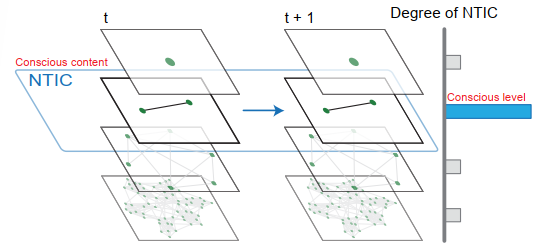
\includegraphics[width=\textwidth]{WritingMaterials/Fig_temp/FoxitReader_2019-01-31_19-03-59.png}
    		\label{fig:LevelOfConsciousness}
    		\caption{Level of coarse-graining and level of consciousness. The degree of NTIC is not a monotonic function of coarse-graining levels, suggesting that high conscious level may exist at a certain coarse-grained level }
		\end{figure}


        
        % -------------  Contents Corresponding to Coarse-grained States ------------- %
		\subsection{Conscious Contents Corresponding to Coarse-grained States}\needfig{maybe I need a figure here}
        As we mentioned above, human conscious contents always consist of rich,  high dimensional, and integrated information. The state space of the correspondent physical system must have the same information capacity as the information content of consciousness.  We claim that conscious contents correspond to the state of the NTIC process. 
        
        This claim implies that the complexity of conscious contents correlates with the amount of information contained in the NTIC process. Therefore, a crucial predict from our theory is that the larger state space of the NTIC process has the richer conscious experience the process can have (e.g., a NTIC process involving a large amount of coarse-grained variables). Crucially, even experience of full darkness contains rich information because it rules out other enormous potential alternative states of conscious contents. Equivalently, in the physical system, to know the state of the NTIC process when there is no sensory input (darkness) also requires the same amount of information from the system. 
        
        Follow the example in the last section\todo{Do I have this example?}, a small creature lives in a simple environment with very limited environment dynamics. It may form a simple NTIC process. However, in this situation, the self-predictive information is very low and the state space of the NTIC process is small. As a result, the richness of the conscious experience this agent has will be very limited. 
        
        Importantly, because the closure is at a coarse-grained scale one state of the informational closure can be mapped to several states at microscopic scale, our theory supports multiple realisation thesis \needref{multiple realisation} which suggests same conscious experiences can be mapped to different physical implementations. 
        
        \begin{WritingMaterials}
    		\begin{figure}[H]
    			\includegraphicsTodo[width=0.8\textwidth]{WritingMaterials/LimitCycle/PhaseCycle.pdf}
    			\label{fig:limitCycle}
    			\caption{Example of coarse-graining by a limit cycle process}
    		\end{figure}
    		
    
    		\begin{equation}\label{eq:LimitCycleExample}
                \begin{array}{l}{\dot{y_1}=y_1-y_2-y_1\left(y_1^{2}+y_2^{2} \right)+\epsilon_{y_1}} \\ {\dot{y_2}=y_1+y_2-y_2\left(y_1^{2}+y_2^{2}\right)+\epsilon_{y_2}}\end{array}
    		\end{equation}    		
    		
    		The noise sources, $\epsilon_{y_1}$ and $\epsilon_{y_2}$, are i.i.d with a normal distribution with mean $\mu=0$ a and variance $\sigma^{2}=1$     
		
        
            @ Our theory naturally explains the com positional nature of consciousness because the joint states of entities in the NTIC process determine the contents of consciousness.

		\end{WritingMaterials}
			
			
			
	    \subsection{Reconciling the levels and contents of consciousness}
	    Segregation of conscious levels and conscious contents raises a debate \citep{bayne2016there, Fazekas2016}. Our framework reconciles conscious level and conscious content. When the information encapsulated in the NTIC process is large and reaches a high NTIC,the system has high level of consciousness. Simultaneously, this provides a rich state space which is equivalent to encoding rich predictive environmental dynamic in the system. From this perspective, levels and contents of consciousness are just two different properties of NTIC processes. An important prediction from our theory is that in which the conscious level is determined by the size of the state space of the NTIC process rather the transient state of a system. For example, when we experience monotonous environment (a dark room), this does not degrade the conscious level.
	    
	    Our framework also explains why in normal physiological states the level and the content are positively correlated \citep{laureys2005neural}\needfig{}. To achieve high NTIC, a system also needs to have high dimensionality and a large state space which guarantees rich and high dimensional information in conscious contents. Therefore, this framework well integrates the two key but debated concepts in consciousness research. 
			
			
			
			\begin{WritingMaterials}
    			@ This implies that, based on the Equation \ref{eq:nticObjective}, the self-predictive information about the future states that the current state holds and the information about the environment encoded in the process determine the level of consciousness.
    			
    			@ This also suggests that the richness of the environment being modelled by the	NTIC process has a direct contribution to the level of consciousness.
    			

				@ To have high level non-trivial informational closure, the states of the coarse-grained scale need to

				@ First, maximise the mutual information between environment and the representation.
				This term implies that the agent need to maximise predictive power of environmental state. This also suggest that the environmental complexity is a crucial factor to the level of consciousness. The more rich and complex environment the agent try to predict the higher level of consciousness the agent has.
				
				@ Consciousness and complexity \cite{Tononi1998}


				@ Second, to minimise the mutual information between environment and the representation conditional on the past state of the representation. This term suggests that the representation is self-predicable and it mimics the environmental transition.

				@ Therefore, this theory predicts that level of consciousness determined by the environment that the agent adapts to. To form a high non-trivial informational closure, the agent will need to live in a complex environment and model the environmental transition precisely.


			\end{WritingMaterials}



		\subsection{sensory hierarchy and neural coarse-graining}\label{sec:SensoryHierarchy}

        It is important to note that the coarse-graining direction is not necessary aligned with \critical{Just saying anatomical is not enough. Need better expression} anatomical sensory hierarchy in the neural system. Our theory is different from consciousness theories which focus on the anatomical hierarchy, for example the intermediate Level Theory \citep[see also \ref{IntermediateLevelTheory}]{prinz2007intermediate, jackendoff1987consciousness}. Due to the pervasive noise in the microscopic levels in the neural system reliable information processes need to be built upon the coarse-grained levels. Nevertheless, to exercise causal power in actuators and environments, information needs to be read out from coarse-grained levels. \needfig{Maybe need a figure discribing brain to hand}. Therefore, the neural system still implement readout decoders for the subsequent signal output. In figure \ref{fig:hierarchy}, the blue arrows indicate the readout mechanisms implemented in the neural system. We argue that previous data suggesting the neural correlates of consciousness between microscopic neural activities and conscious contents may be misled. 

        
			\begin{figure}[H]
				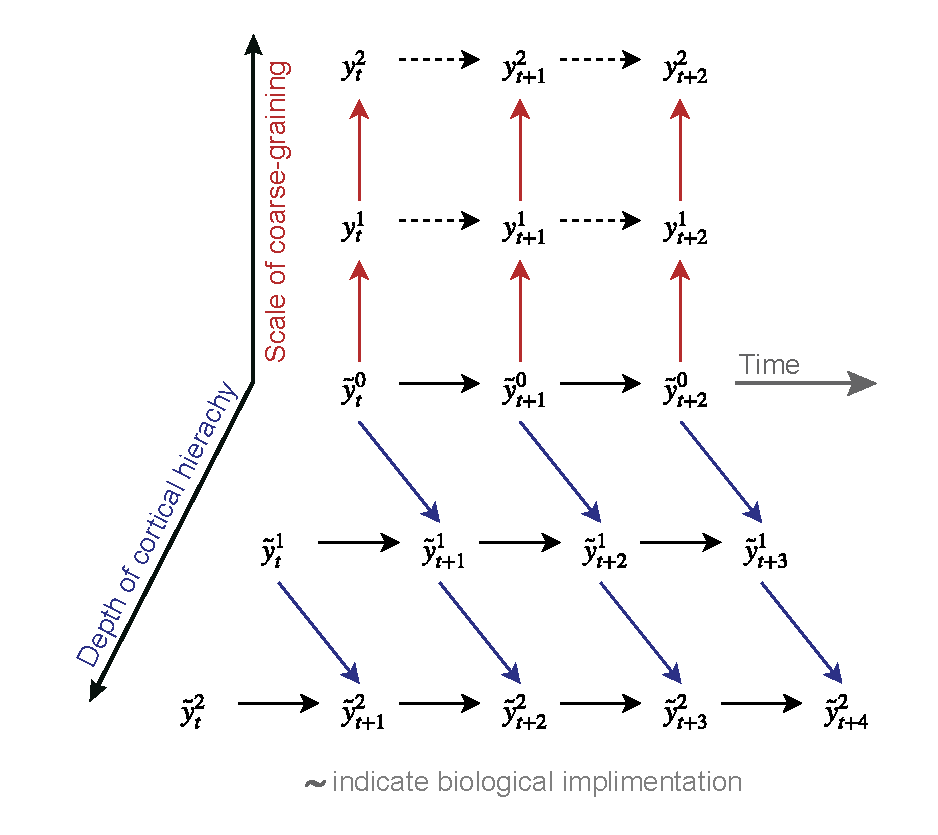
\includegraphics[width=\textwidth]{WritingMaterials/Fig_SeperationOfCGandCortHierachy/SeperationOfCGandCortHierachy.pdf}
				\label{fig:hierarchy}
			\end{figure}


            \begin{WritingMaterials}
    			@ Of course, from evolutionary perspective, neural system should develop a better hardware to support neural coarse-graining

				@ For example, pooling layers in CNN is an implementation of coarse-graining function. It' is very plausible visual processing hierarchy in the neural system realises pooling layers.


				@ It is possible that the neural system represents higher-level information processing by low level physical subtract. For example, studies have found representation for summery statistics of signal and neural. population.\needref{neural representation for summery statistics}\\
				From this point of view, sensory hierarchy may extend along with levels of coarse-graining.
            \end{WritingMaterials}
        


        \subsection{Dynamical Boundary}
        Our theory predicts that the boundary of a conscious system is dynamical. The boundary is determined by elements forming high NTIC. This implies that when the structure of interaction between elements changes the physical boundaries supporting consciousness should also change. If some coarse-grained variables encode environmental information, they may become necessary components to form high NTIC. In such case, these coarse-grained variables are "recruited" inside the boundary of conscious processes. Note that, due to synergistic information, even recruiting some new variables may largely increase the level of NTIC. 
        This may explain why consciousness is tightly associated with binding and integration of information in human perception and cognition. Another crucial implication is that the same neural substrates may not be always involved in conscious processing rather it depends on whether it creates high NTIC with other members in the neural system. \needfig{Maybe I need a figure here as well}
    
    
% ============================================================================ %
%                    Conscious versus Unconscious Processing                   %
% ============================================================================ %
	\section{Conscious versus Unconscious Processing}\label{sec:Conscious versus Unconscious Processing}
	    In this section, we show how our theory can make predictions about whether a process is conscious or unconscious. While our theory is built upon a minimal set of assumptions, it possesses predictive power about the relationship between information processing in the neural system and conscious experience.
	    
		Our theory argues that, to make information conscious, the following necessay and sufficient conditions need to be satisfied.
		
		\begin{enumerate}
		    \item Sufficient condition: Information is encoded in NTIC process. 
		    \item Necessary condition: The system is capable of constructing NTIC processes at coarse-grained levels. 
		\end{enumerate}		
		
        We especially highlight the second condition because it is critically related to many empirical research results even though it is only a necessary condition. As we will describe below, this theory can well explain a varieity of previous empirical findings in consciousness science and further make predictions for future research. In this section, we discuss how the two informational-based conditions link to conscious experience. 
		
		
		
        % ---------------------------------------------------------------------------- %
        %                            Unconscious Processing                            %
        % ---------------------------------------------------------------------------- %
        \subsection{Unconscious Processing}
        
        \subsubsection*{Fail to meet the 1\lowercase{st} condition}
            If a process fails to fulfil either of the two conditions, information remains unconscious. We first consider the scenario that a process fails to satisfy the first condition, i.e. the process fails to achieve high degree of NTIC. In the neural system many processes fall into this category. 
        	
        	Considering the objectives of achieving NTIC (Eq. \ref{eq:nticObjective}), if a process is unable to maximise the mutual information between its past and future states ($I(Y_{t+1};Y_{t})$), it results in low NTIC. The failure to maximise the mutual information implies the past states of the process itself has little influence on its future states. In the meantime, if environmental information is able to flow into the process, the process can still produces functional outputs based on the current state of the environment accordingly. However, in this circumstance, the future state of the process is largely determined by the environmental states. That is, the process is not informational closed (${J_{t}(E \rightarrow Y )} \not\approx 0$, Fig.\ref{fig:reflexive}). 
            	
            % or minimise $I(Y_{t+1};Y_{t}|E_{t})$
            	
            % If the future states of the system have strong mutual information with the current environmental states ($I(Y_{t+1};E_{t})$) but have weak mutual information with the current system states ($I(Y_{t+1};Y_{t})$), the informational closeness will be small.
                
        	% reflexive behaviour
    		\begin{figure}[H]
    			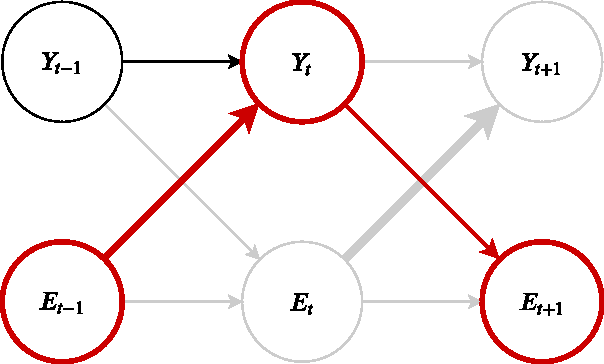
\includegraphics[width=0.8\textwidth]{WritingMaterials/Fig_Reflexive/Reflexive.pdf}
    			\caption{Reflexive Behaviours}
    			\label{fig:reflexive}
    		\end{figure}        
            
            In the neural system, this type of processes, for perception, shows the property that the perceptual processing mainly passively responds to the sensory inputs. For actions, this type of processes only produces "reflective-like" behaviours. Reflexive behaviours are commonly considered as automatic and non-conscious behavioural controls \citep{casali2013theoretically}\needref{More referene}. We argue that information carried by this type of processes is unconscious due to its failure of achieving high NTIC, i.e., the first condition. 
            
            The same principle can be applied to blindsight and procedure memory \needref{blindsight} which are often considered as unconscious processing. Blindsight patients are able to track objects, avoid obstacles, and make above chance-level judgements without having any conscious perception about visual stimuli. We believe that these behaviours can be guided by direct stimulus-response mappings ($S\rightarrow{}R$). However, the direct $S\rightarrow{}R$ mappings also lead to non-NTIC neural processes  and, therefore, are unconscious. Similarly, in the case of procedure memory, processes always rely on both the current environmental and system states to determine the next state of the processes\needref{Do I need ref??}. The information flow from the environment to the system is crucial to guide the state transition of procedural memory. Therefore, information processing of procedural memory also fails to achieve high NTIC and remain unconscious. 
            
             This type of processing is similar to the model-free policy-based agents in the reinforcement learning framework. The agent learns a policy $\pi$ which directly maps sensor values $S$ to output action $A$.
        % @ $\pi : S \times A$\\
        % Policy
    		\begin{equation}
    			\label{eq:PolicyBasedAgent}
    			\begin{aligned}
    			    \pi(A | S)=\operatorname{Pr}\left(A_{t}=a | S_{t}=s\right)
    			\end{aligned}
    		\end{equation}
    		
    		Our theory can explain why the patients with visual apperceptive agnosia (e.g., the famous case D.F.\cite{james2003ventral}) can perform online motor controls without visual awareness of action targets \citep{10.3389/fneur.2014.00255}. The online visual information can be used to perform functional actions without forming a NTIC process. Our theory also explains why unconscious processes in this category often fail when a long delay periods is introduced in the tasks. Without self-predictive information in NTIC, the policies of motor outputs largely depends on the present environmental and sensory states implying that this type of processes often can only work online. With a long, sensory information is unable to guide the delayed motor outputs and leads to failure consequences. 
    		
    		Finally, an interesting implication from our theory is that a pure feedforward neural network cannot be conscious because it is unable to maintain any form of memory so that there is no influence from the system past states to its future state. In contrast, with recurrent loops, a neural network is able to create information channels from its past to its future states and becomes capable of achieving NTIC. This result coincides with some theories of consciousness which emphasize the importance of recurrent circuits to consciousness \citep{lamme2006towards, edelman1992bright, tononi2008neural}.
    		% if more references are needed, check Eklund_2012_RECURRENT PROCESSING AND THE CONSCIOUSNESS.pdf
    		However, we derive this conclusion from a more fundamental informational-related hypothesis indicating the more generalised principle behind it. 

        % ---------------------------------------------------------------------------- %
        %                                Fail to meet 2                                %
        % ---------------------------------------------------------------------------- %

        \subsubsection*{Fail to meet the 2\lowercase{ed} condition}
        As mention above, information is level-dependent and can be virtually independent (closed) across different coarse-graining scales. If processes at some levels of a system are able to achieve high NTIC and become conscious, information at other levels still remains unconscious. The first implication of this argument is that processes at levels with high stochasticity are unable to achieve high NTIC and, therefore, unconscious. High stochasticity corrupts informational channel capacity and leads to low mutual information between past and future states of a process. In the neural system, the cellular level activities are highly noisy and are unable to reach high NTIC. Therefore, the information processed by the microscopic levels in the neural system are not conscious and we never can experience detail activities in the microscopic levels. 
        
        
        We argue that many mysterious results in previous research of consciousness are originated from inappropriate biological and behavioural measurement scale. In the following, we list some examples. 
        
        
        Unconscious processing in this category of 
        
        @ Evidence suggests that the neural system is able to encode probability distribution and perform probabilistic inference in a near optimal way\needref{bayesian brain}. However, an intriguing fact is that we are nearly ignorant of all the probabilistic computation of the inference processes but are only aware of "a sample" of the posterior distributions of the inferences \citep{dehaene2017consciousness, vul2009attention, asplund2014attentional, vul2008temporal, moreno2011bayesian}. The information of all alternative possible states is unable to enter conscious contents. In short, one needs to explain why the neural system can hold the joint probability distributions of inferred variables but, however, only a realisation of the inference outcome becomes conscious. Based on our theory, we argue that the computation of statistical inference is carried out at microscopic levels of the neural system and the NTIC process correlated with conscious contents only possesses the coarse-grained information of the computation. The mapping from the microscopic to macroscopic states naturally leads to a single and stable state at the macroscopic levels.
        
        For example, Fig. \ref{fig:TemperatureExample} illustrates the relationship 
        At the left panel, two cups contain water with different volumes $V_t$ and temperatures $T_t$. Even though we know volumes and temperatures are coarse-grained macroscopic variables, the states of mixed water ($V_{t+1}$, $T_{t+1}$) can still be predicted without knowing any information from the microscopic levels (the molecular level),i.e., the information closure at the macroscopic level. Similarly, taking Bayesian inference as an example, the microscopic neuron populations are able to represent probabilistic distributions about inferred target variables and the neural networks perform the statistical inference to obtain the posterior distributions. However, enormous microscopic neural states can be coarse-grained into the same state of summary statistics (e.g., the mean $\mu_{t}$  and standard deviation $\sigma_{t}$) at a macroscopic level. The state transition ($\mu_{t+1}$ and $\sigma_{t}$) is also predictable without any additional information from microscopic levels. Therefore, consciousness can only "observe" the coarse-grained states without the knowledge of how the statistical inference is implemented and performed at the microscopic levels. 


		\begin{figure}[H]
			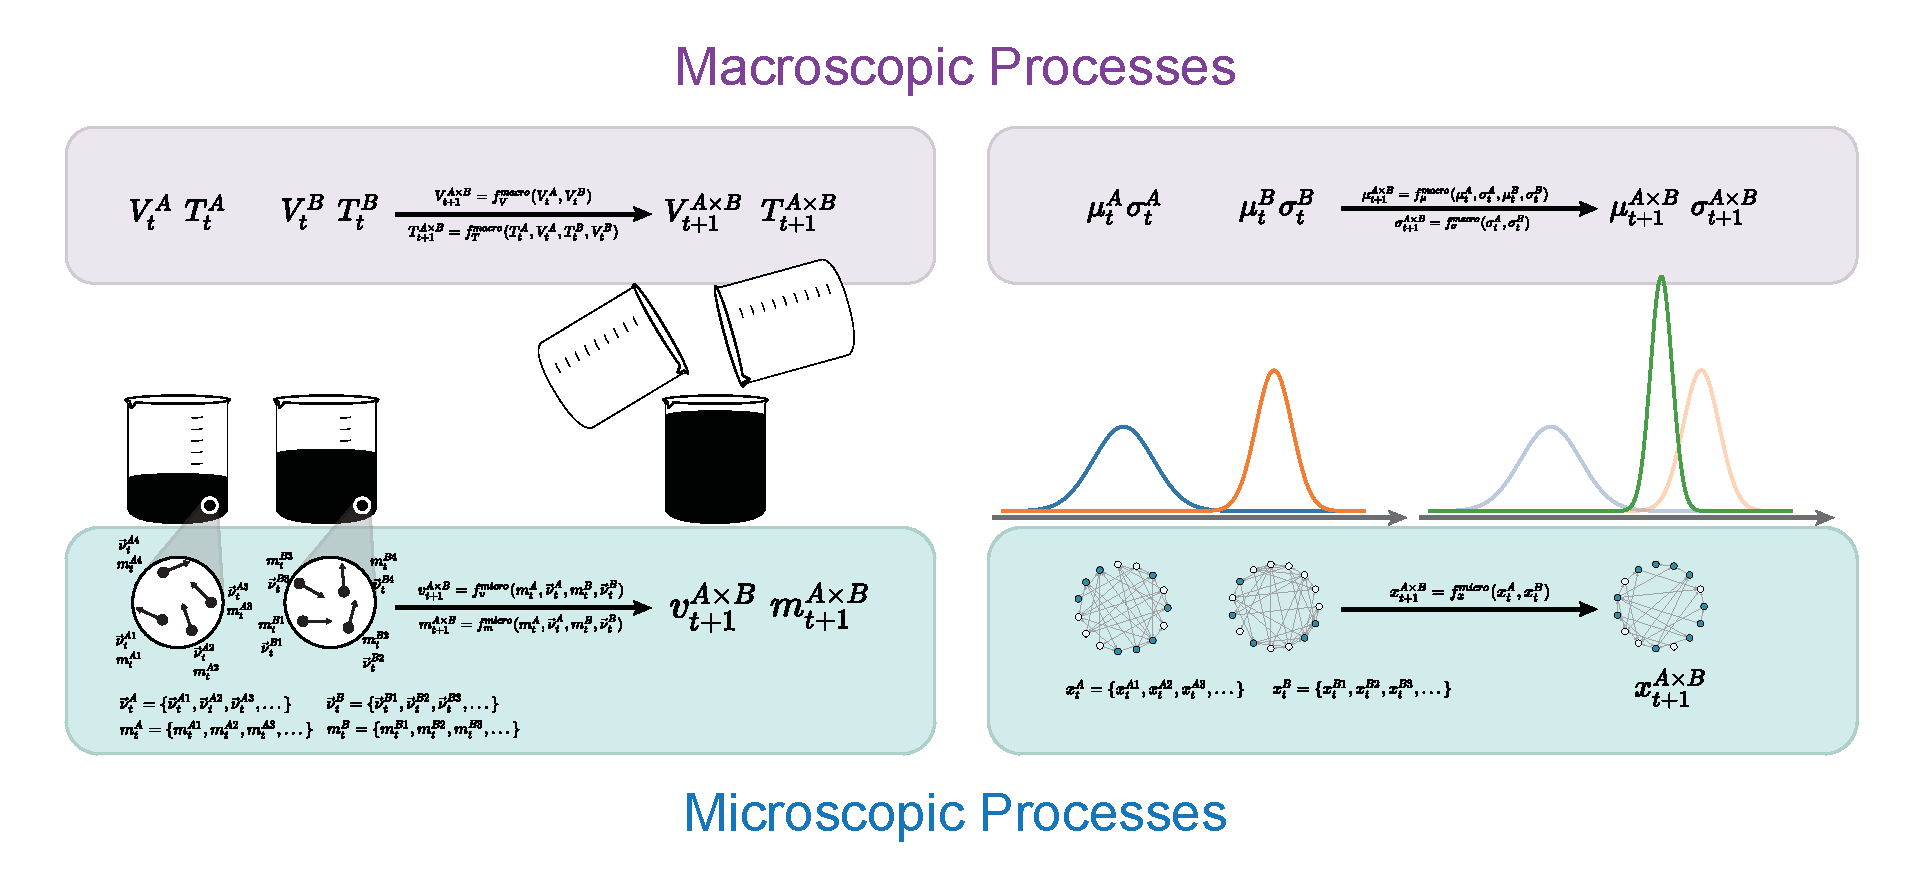
\includegraphics[width=1.3\textwidth]{WritingMaterials/Fig_Temperature_Example/ExampleOfCG.pdf}
			\centering
			\caption{An Example of ...}
			\label{fig:TemperatureExample}
		\end{figure}         
        
        
        The same scenario can be applied to the results from Libet's volition experimental paradigm \citep{Libet1983TimeOC, Libet1985Dec}. Experiments using similar procedures usually show that the recorded neural activities start earlier than subjects' feeling of their own intention to act in the self-determined experimental settings. We argue that free actions are initiated at the microscopic levels, for example, the random fluctuation in the neural system \citep{schurger_accumulator_2012}. However, the conscious experience of volition is information at the macroscopic level with NTIC. Due to the information closure, there is no way for the NTIC process to observe the information of the microscopic states, i.e. the initiation of actions. 
        
    
        \idea{Not sure if I want to address this point}  Note that, some evidence suggests single-cell-level correlation of conscious experience, the Jennifer Aniston cell for example \citep{Quiroga2005Jun, Quiroga2012Jul}. This may seem to counter our argument that single-cell level information is incapable to be conscious. However, first, the correlations are always not the direct microscopic state changes of the cells, e.g. the action potentials. Instead, the correlated variables are always coarse-grained. The neuronal firing rate, for example, is a temporal coarse-grained variable. Second, it has been well established that heterogeneous nonlinearity is critical for neural populations to encode rich and high dimensional information. \citep{Chelaru2008, Rigotti2010Oct, Shamir2004Jun}. It is common to detecting a single neuron whose activity profile well align with a subspace which represents a single object within the state space of a population code.\needhelp{Maybe need to rewording here} We believe that multi-scale data and analyses are needed to elucidate whether single neuron behaviours are sufficiently representative for any type of conscious experience. 

        
        

		
		\begin{WritingMaterials}
        	@ \idea{Should I write the following points? Is this too much?}
        	@  === boundary conditions  === 
        	% multistable perception
        	    @ In the case of multistable perception, at every moment, only a single macroscopic state is mapped from the microscopic levels, we can only be aware of one interpretation at every moment. 
        	    
        	    
        	% Priming
        	    @ The same mechanism can also applied to unconscious priming effects. \highlight{Making state transitions at microscopic levels does not guarantee transitions at macroscopic levels.}\ideaCallout{this is the key sentence}
        	    
        	    @ Of course, this is related to what kind of coarse-grain function which can form a NTIC process at macroscopic scales. We will discuss this issue in the later section.
        	    
        	   
        	   
        	   
        	   @ The third category is the boundary conditions. 
        	   
        	   % Binocular rivalry
        	   @ In binocular rivalry, either eye provides information to form a NTIC process. Once the process is NTIC, the process continue the trajectory in the state space and close system. Information from the other eye is unable to enter the process, thus it remains unconscious. 
        	   
        	   @ Including information from either of objects information can achieve NTIC. 
        	   
        	   @ For example, when the information of the visual stimuli both can form the NTIC.
        	   
        	   @ Our theory also explains why the conscious percepts show some kind of inertia (stably remain conscious for a period of time). 
        	   
        	   @ Once the NTIC process is formed, the closureness guarantees the stability of the state transitions of the process. 
                
            \end{WritingMaterials}
        
        


		
		\subsection{Conscious Processing}
		When the both conditions are fulfilled, our theory suggests that the states of a NTIC process correspond to particular conscious contents and the information incorporated in the NTIC process is conscious. Due to the predictive nature about the environment dynamics of NTIC processes, to achieve high NTIC and to construct functions within the process have a huge evolutionary advantage. It is important to emphasise that our theory does not suggest any functionalism of consciousness. Rather, we argue that information fundamentally associates with consciousness. Nevertheless, consciousness research still suggests a strong functional relation between consciousness and some specific types of cognition and behaviours \citep{Seth2009Encyclopediaofconsciousness}. We believe that this relation comes from several special properties of NTIC and these properties support the foundations of many cognitive functions in the neural system.
		
		First, a NTIC process encodes predictive information about environmental dynamics. This is crucial for constructing forward models for predicting future states of the environment. Therefore, cognitive functions which require agent-scale prediction are likely to be accompanied by conscious experience. This properties is required by planning and also achieving long term goals.\needref{}
		
		Second, a NTIC process can be considered as a close form simulation machine. With a given initial state, the process can self-evolve and follow a certain trajectory in the state space. This trajectory can be seem as a simulation about the environmental transition. Therefore, a NTIC process can serve cognitive functions as a perfect simulation engine \citep{BERTSCHINGER.2006}. Accordingly, mental simulation, imagination, computing alternative realities, and generating counterfactual outcomes can be implemented with a NTIC process. \needref{}
		
	    Third, an important properties of NTIC processes is its high stability. The state transitions and trajectory are highly predictable. In such case, NTIC processes are more suitable for integrating information across larger time scales (above millisecond). Therefore, tasks which require to integrate information across time above the millisecond scale are often associated with conscious experience. 
	    
	    Fourth, a NTIC process as a closed system can still provide predictive information without new information flowing into the process. This is crucial for many types of off-line processing. 
	    
	    Fifth, any state of a NTIC process can be seem as a integration of multiple sources of information. For the human scale activities, to know certain transition about the environment, the NTIC process must include a high dimensional information from multiple modalities and have the knowledge about how the high dimensional data interact to each other. Without the knowledge and information, a process may not be capable of produce a stable state transitions which mimic the environmental dynamics. Thus, cognitive functions requiring this large scale integration are likely to be conscious. Furthermore, the high dimensional integrated information is also critical for an agent to learn new behaviours to achieve flexibility and the strategic behavioural controls and decision-making. 
	    
	    In sum, we argue that having a NTIC process is critical for survival in the evolution. It is likely that biological creatures acquired NTIC process at some stages in the evolution. And due to the fundamental relationship between information and consciousness, these biological agents also acquired different degrees of consciousness depending on the physical scales and the complexity of the environments they live in. Our theory well explains why some processes and functions in the neural system are conscious and some are not with only two parsimonious conditions. 
		
		\begin{WritingMaterials}
		    @ Previous research has identified a set of perceptual and cognitive functions which not exclusively but frequently associate with consciousness. 
		    
    		    @@ Planning, achieving long term goals
    		    
    		        @@@ simulate alternative realities 
    		        @@@ multiple alternative possibilities
    		        @@@ imagination
    		        @@@ information for off-line processing
    		    
    		    @@ Cognitive control, response inhibition, flexible routing of information, overriding automatic responses
    		    
    		        @@@ flexibility and the strategic use of that information for complex operations and decision-making 
    		        @@@ flexible and adjust our behavior to different contexts and goals
    		    
    		    @@ integration,
    		    
    		    @@ integrates behaviour across time
    		    
    		        @@@ tasks for long duration
    		    
    		    @@ stabilisation
    		    
    		    @@ conscious thought, reflection, reasoning, and temporally extended sense of self. 
    		    
    		    @@ complex visuomotor abilities
    		    
    		    @@ intending deciding
    		    
    		    @@ dreaming
    		    
    		    @@ reasoning interpreting
    		    
    		    @@ self
    		    
    		        @@@ reflecting
    		        @@@ self-monitoring 
            @ As mentioned in \ref{sec:Non-trivial informational closure}, achieving NTIC has a large evolutionary advantage. 
            
                @@ Because NTIC processes encode information about environmental transition, it becomes a perfect computational core for constructing forward models for the environment, simulating the dynamics of self-environment interaction, and generating predictions. 
                
            @ Therefore, if an agent equips a NTIC process, the process can be used to integrate information from different sources. 
            
            @ =============================================================================
            
	        @ importantly, evidence suggests that those functions in some conditions do not require the involvement of consciousness. This evidences an important fact that consciousness is not necessay to these functions. 
	        
	        
	        @@ Predictive information about the environment.
	        
	        @@ Stability 
	        
	        @@ simulation environmental dynamics 
	        
	        @ Replaying past events
	        
	        @ \rewrite{However, recent evidence also points out interesting dissociations between conscious and unconscious information processing when it comes to the duration, flexibility and the strategic use of that information for complex operations and decision-making} \cite{van2012role}
	        
	    \end{WritingMaterials}
	    


% ============================================================================ %
%                        Comparison with other theories                        %
% ============================================================================ %
	\section{Comparison with other theories}
	In this section, we compare our theory with other popular modern theories of consciousness. 1

		\subsection{Theories about multilevel views on consciousness and cognition}
		Previously, similar to our theory, several multilevel views on consciousness and cognition have been proposed. We shortly discuss two theories relevant to our current proposal.
            \subsubsection*{Level of Organisation \cite{wimsatt1994ontology}}
                As mentioned previously, the level of coarse-graining is different from the anatomical level.
                Pennartz focuses more on multimodal representation as the most important factor (See the discussion in \cite{pennartz2015brain}). Our proposal is inline with Pennartz's Neurorepresentational  theory (Neurorepresentationalism) \cite{pennartz2018consciousness,pennartz2015brain}. However, it’s crucial to note that our theory claims only the level of coarse-graining achieving NTIC matters to consciousness rather than the anatomical level of sensory hierarchy. 

			\subsubsection*{Intermediate Level Theory} \label{IntermediateLevelTheory}
                One important theory tries to connect consciousness to multilevel views is the Intermediate Level Theory (ILT, \cite{jackendoff1987consciousness, prinz2007intermediate}). ILT proposes that conscious experience only correlates specific levels of representations in the hierarchy of sensory processing. ILT claims that consciousness only associates with the representation at intermediate levels (e.g., the 2.5D representation in terms of visual processing) rather than the ones at lower-level or higher-level. 
                One fundamental difference between ILT and our theory is the definitions of the level. In our theory, level is within the context of coarse-graining. However, ILT focuses more on the levels in terms of anatomical direction (see fig \ref{fig:hierarchy}). As mentioned previously, we emphasise that we doesn't assume the direction of coarse-graining should align with the direction of anatomical processing levels along cortical hierarchies. This leads to an important difference that the level of coarse-graining exists virtually. However, the level of cortical representation should be referred to neural substrates. Finally, different from ILT which suggests that some neural substrates responsible for the 2.5D computation are conscious, we predict that once information carried by coarse-grained variables is involved in the NTIC process, brain areas, not exclusively within 2.5D representation, should  co-vary with conscious contents. 
				
			\subsubsection*{Pennartz's neurorepresentational theory (Neurorepresentationalism)}
			    Our theory shares some close concepts with Pennartz's Neurorepresentationalism \citep{pennartz2018consciousness,pennartz2015brain}. Similar to Neurorepresentationalism, our framework is also close to Marr's original distinction between the levels of analysis \citep{marr1982vision, pennartz2015brain, pennartz2018consciousness}. However, a fundamental difference between the two theories is that Neurorepresentationalism takes more functionalist point of view and suggests NCC should serve high-level world-modeling and makes a best guess about the interaction between the body and the environment. Neurorepresentationalism also suggests conscious experience is associated with integrated representation for multimodal and situational information. Out theory suggests that the association between the functions mentioned in Neurorepresentationalism is rooted in the more fundamental relationship between information and consciousness in which NTIC plays an important role. 
	
		       
		        \begin{WritingMaterials}
				%% Back up materials
				
				@ Prinz suggested that \rewrite{as. Cells in V1 are not promising candidates, because they do not reliably respond in ways that are consistent with features that we experience consciously. } \cite{prinz2007intermediate}
			    
				@ \rewrite{
					The intermediate level theory originally proposed by Ray Jackendoff and further defended and specified by Jesse Prinz proposes that within the hierarchy of representations that are used to describe the cognitive system, conscious experience occurs only for specific levels of representation. The theory is rooted in Jackendoff ’s analysis of different cognitive systems such as vision, language, and music and the subsequent observation that consciousness does not arise anywhere within these systems. According to Jackendoff, consciousness is not associated with low-level, nor with high-level representations, but rather with those implying intermediate levels of processing. For instance, in the domain of object recognition, it is assumed that the visual system comprises a low level with local computations of visual features, an intermediate level reflecting binding and object recognition, and a higher level computing viewpoint invariance and representing abstract categories. According to Jackendoff and Prinz, conscious experience is not comprised of a disunified picture of visual features, nor is it represented by viewinvariant categories. Rather it is composed of bound and specific instances of objects that are assumed to be computed at the intermediate level of representation. In an analogous manner, speech perception can be decomposed into three levels: an acoustic representation of speech sounds at the lower level, a high level involving abstract lexical and syntactic categories, and in between a word recognition level relying on phonological representations. This theory explains why the conscious experience associated with speech perception mostly involves phonological representations, rather than other levels of representations. In Jackendoff and Prinz’ theory,the privileged role of the intermediate level of processing is based on the need for real-time computational efficiency. Indeed, this level of representation is assumed to be the most relevant one regarding ecological and functional needs. Another important aspect of this theory concerns the central role of attention during conscious experience. Here, attention is defined as a selection process that acts as a gate to working memory mechanisms. It performs the function of selecting the relevant information that is amplified afterward and then becomes conscious. Indeed, Prinz acknowledges that activation of an intermediatelevel representation on its own cannot be a sufficient condition for consciousness, given that those representations can be activated during subliminal perception. However, this theory makes the crucial postulate that the amplification of intermediatelevel representations by attention is a necessary and sufficient condition for consciousness. In sum, for each domain of processing, the content of consciousness at a particular moment is supported by a representational structure of intermediate level for that domain, which is selected to enter short-term memory, and enriched by attentional processing.} \cite{banks2009encyclopedia}

				@ \rewrite{
					In 1987, Ray Jackendoff published Consciousness and the Computational Mind. In it, he posed an important Where question: Where, in the fl ow of information, does consciousness arise? Most cognitive scientists agree that the mind is, in some sense, a computer. It is a device that processes information by transforming representations in accordance with rules. Computational devices decompose into various interconnected subsystems, each of which performs some aspect of a complex task. Given such a decompositional analysis, we can ask: in which subsystems does consciousness arise? If we depict the mind as a vast fl ow chart, and highlight the boxes whose rules and representations are conscious, which boxes should we mark? Jackendoff ’s answer is simple and elegant. He noticed that many of our mental capacities, including our senses and our language systems, are organized hierarchically. In each of these hierarchies, it makes sense to talk about low- , intermediate- , and high- level processing systems. We break down tasks into stages. Appealing to prevailing models of these stages, Jackendoff observed that the intermediate level seems to be privileged with respect to consciousness. Consciousness seems to arise in intermediate- level processing systems and not elsewhere.} \cite{prinz2007intermediate}

				@ \cite{jackendoff1987consciousness}
				@ \cite{prinz2007intermediate}
				@ 2.5D


				@ about why it is this level
				@@ \rewrite{
					Under the computational interpretation, the “why” question means: In what sense are intermediate level representations computationally important or distinctive? Th is is a tractable question, and it may lead to insights into the function of consciousness. Representations at the intermediate level are ideally suited for real- time deliberative behavioral responses. Low- level representations fail to bind features into coherent wholes. If we are going to interact with our environment, the low level is not a good guide. Th e high level is a good deal better for action, but also suboptimal. Th e high level tells us the category of the stimuli we perceive, but from an allocentric point of view. It abstracts away from stimulus features that are crucial for action. If we encounter a predator, the high- level visual representation does not tell us if it is facing toward us or away from us. Without that knowledge, we cannot decide what course of action to take. So, I propose that the intermediate level plays a distinctive role in information processing. It delivers representations that are coherent but viewpoint specifi c. Th ese representations are useful for determining what to do here and now.arg1} \cite{prinz2007intermediate}
				@@ \rewrite{
					I conclude that the intermediate level plays a distinctive and important computational role. Some researchers find this puzzling. In wondering why the intermediate level is privileged, they note the arbitrariness of the fact that perceptual hierarchies have three levels. Could they not have two? Or a hundred? Do the 50 or so areas that contribute to visual processing really divide neatly into three levels? I think these puzzles depend on a particular understanding of what the word “intermediate” amounts to. One might get caught up in the fact that the intermediate level is the second stage in a sequence. Call this the “serial understanding of the intermediate level.” Alternatively, one might think of the intermediate level semantically. On this reading, the intermediate level is one that is not abstract and categorical, but not piecemeal or disunifi ed. Th ese notions are all in need of some refi nement, but, as a fi rst approximation, the idea is that intermediate- level representations are neither too specifi c nor too general.}\cite{prinz2007intermediate}
			\end{WritingMaterials}

		\subsection{First-order theories}
            The first-order theories suggest that consciousness is determined by early sensory information or neural activities\needref{First-order theories}. The first-order view maintains that conscious awareness is determined by early sensory activity alone, independently of higher-order representations.
            First-order theories suggests that phenomenal consciousness is associated with fine-grained contents for the first-order processes. Different from the first-order theories, our theory suggests that, whether the early sensory activities show in the conscious content, it depends on information encoded in the early sensory areas is recruited in the NTIC process at the macroscopic level or not. As we mentioned in \ref{sec:Unconscious Processing}, if the sensory activities are only passively triggered by the environmental states, they are not able to form hign NTIC and remain unconscious. We predict that, if early sensory information or neural activities after coarse-graining take parts in the NTIC process, early sensory information or neural activities can contribute conscious content. 
		
		
			\begin{WritingMaterials}
				@ \rewrite{
					The first-order view maintains that conscious awareness is determined by early sensory activity alone, independently of higher-order representations. Thus the crucial difference between the first-order and higher-order views is that the latter but not the former predict that conscious awareness is determined at least in part by prefrontal and parietal activity. Therefore, in the group of first-order theorists we include here not only those commonly labeled as such in the philosophical literature [11] but also theorists, such as Ned Block [12,13], who hold that the phenomenal qualities of awareness depend on the biological substrate rather than merely the content of the first-order representations, as well as scientists who hold that visual awareness depends on activity in content-specific regions of the extrastriate cortex [24,25] or on feedback from these regions to the primary visual cortex [26]. Most first-order theories explain the difference between awareness and unawareness by positing that the latter is associated with weak information [29] or with representations in alternative (e.g. subcortical) sensory pathways. Thus this view suggests that conscious and unconscious processing will have different functional consequences. Whereas some first-order theorists hold that some higher cognitive functions can be performed without conscious awareness [30–32], most first-order theorists take a difference in perceptual task performance (e.g. ‘hits’ vs ‘misses’ in a detection task) as evidence for a difference in conscious awareness [12,13,25,26,33]. In other words, they typically associate task performance with awareness..} \cite{lau2011empirical}

				@ Among those are first-order theories, on which a mental state is conscious if being in that state results in one's being conscious of something;


				@  According to first-order views, phenomenal consciousness consists in analog or fine-grained contents that are available to the first-order processes that guide thought and action. So a phenomenally-conscious percept of red, for example, consists in a state with the analog content red which is tokened in such a way as to feed into thoughts about red, or into actions that are in one way or another guided by redness.
				
				@ However, due to coarse-graining, changes of early sensory information or neural activities do not necessarily accompany with changes of conscious contents. \todo{Need more here, espectially more counterintuitive predictions}

			\end{WritingMaterials}
			
			
		\subsection{Higher Order Thought theory of consciousness}
		    \ideaBox{Okay, I don't know how to deal with HOT now. I don't understand it at all}
		    In contrast to first-order theories, higher-order thought theories suggest that consciousness depends on higher-order representations which represent agents as being in particular internal states \citep{lau2011empirical}. First-order processing needs to be observed or represented by a higher-order observer to become conscious. 
		    
		    
		    Meta-cognition is also associated with many conscious cognitive function. However, we propose a new perspective and indicate that HOT may be a misunderstanding \critical{Very bad writing. I need to rewrite this part}. 
		    
		    
		    This may be the result of neural coarse-graining. Because contents in informational closure look like watching fine-grained information, people may have an wrong impression about it. 
		    
		    
		    Coarse-grained information can be summary statistics which may be misunderstood as higher-order representation. It is true that the neural system does create  meta-representation to represent xxx\needref{Maybe come studies about confidence represenatation}. The higher-order representation may resemble coarse-grained variables. This may cause misidentify the entity which correlates conscious experience.  
		    
		    Moreover, the predictive information in NTIC is critical for other systems to build forward models for a wild range of tasks. Therefore, most of the high level cognition can utilise the state of informational closure. For example, mental planning needs a precise forward model to infer the environmental dynamics.


			\begin{WritingMaterials}
			@ Good reference: \myQuote{Higher- Order Th eories of Consciousness; PETER CARRUTHERS (The Blackwell Companion to Consciousness (Blackwell, 2007))}

		    @ In contrast to first-order theories, higher-order thought theories suggest that consciousness depends on higher-order representations representing agents as being in particular internal states.
		    
		    @ Coarse-grained information can be summary statistics which may be misunderstood as higher-order representation.
		    
		    @ It is true that the neural system does create  meta-representation to represent xxx.\needref{Maybe come studies about confidence represenatation}
		    
		    @ The higher-order representation may resemble coarse-grained variables.
		    
		    @ This may cause misidentify the entity which correlates conscious experience.  
		    
		    
		    
		    @ ----------------------------------------------------------------------------
		    
			@ Information closure directly is critical for other systems to construct forward models.

			@ Therefore, most of the high level cognition can utilise the state of informational closure.

			@ For example, mental planning needs a precise forward model to infer the environmental dynamics.

			@ \idea{This is way HOT always involve consciousness }

			@ \cite{rosenthal2005consciousness}


            @ ============================================================================

			@ \rewrite{
				According to this view, humans not only have first-order non-conceptual and/or analog perceptions of states of their environments and bodies, they also have second-order non-conceptual and/or analog perceptions of their first-order states of perception. And the most popular version of higher-order perception theory holds, in addition, that humans (and perhaps other animals) not only have sense-organs that scan the environment/body to produce fine-grained representations that can then serve to ground thoughts and action-planning, but they also have inner senses, charged with scanning the outputs of the first-order senses (i.e. perceptual experiences) to produce equally fine-grained, but higher-order, representations of those outputs (i.e. to produce higher-order experiences). A version of this view was first proposed by the British Empiricist philosopher John Locke (1690). In our own time it has been defended especially by Armstrong (1968, 1984) and by Lycan (1996).} \url{https://plato.stanford.edu/entries/consciousness-higher/#SelRepHigOrdThe}

			@ \rewrite{
				neutral about whether conscious awareness adds significant utility or immediate impact on behavior and task performance [1,27]. This is because the view assumes that task performance in most perceptual and cognitive tasks depends mainly on first-order rather than higher-order representations. Because conscious awareness can differ even if all first-order representations remain completely unchanged, such awareness itself might serve little function [1,27].}\cite{lau2011empirical}
				\ideaCallout{
					My theory would have similar prediction. Because conscious contents are coarse-grained results from low-level information. It is possible that more than two low-level neural states all coarse-grained to a high-level state.  }
					
			@ \rewrite{
					Metacognition: cognition that is about another cognitive process as opposed to about objects in the world. In this article we use it mainly to refer to sensory metacognition: a cognitive process that concerns the quality or efficacy of a perceptual process. The capacity of sensory metacognition is sometimes empirically assessed by the correspondence between subjective report and task performance: how closely are they associated with each other on a trial-by-trial basis}\cite{lau2011empirical}
					
			\end{WritingMaterials}

				
        % ---------------------------------------------------------------------------- %
        %                            Global workspace theory                           %
        % ---------------------------------------------------------------------------- %
        
		\subsection{Global workspace theory}
		\needhelp{I think I need some help here. I am not sure what should I write here. Or  what position I should take. To some extent, GWT is a very qualitative theory. It kind of just summarises everything. Without any modelling work on NTIC, it's difficult to say whether we will replicate those profiles of consciousness mentioned in GWT.}
		\ideaBox{Need ending and better difference }
		Global workspace theory (GWT; \cite{baars1988cognitive, baars1997theatre, baars2002conscious}) or Global Neuronal Workspace theory (GNWT; \cite{dehaene1998neuronal, dehaene2001towards, dehaene2011experimental}) states that the neural system consists of several specialised modules and a central global workspace (GW) which integrates and broadcasts information amount these modules. Only the information accessed by the global workspace can be consciously aware of. These modules competes with each other to gain the access to the GW and the information from the winner can trigger an all-or-none "ignition" in the GW. Information in the GW is able to be broadcasted to other modules. Conscious contents then associates information which gains access to the internal global workspace \cite{Dehaene2017}.
		
		In many aspects, our theory can well accommodate GWT. NTIC processes shares several properties with the GW. Here we discuss three core properties, stability, broadcasting, and non-linear ignition, emphasised by the GWT. 

		% === Stability ===
		Stability: GWT indicates that the conscious contents often show stronger stability which may be necessary for the neural system to integrate information from a variety of modules. Suggested by GWT, this is caused by top-down amplification from the GW to individual modules which gain the access to the GW \needref{}. In contrast, without assuming any additional mechanism, our theory argues that stability is a natural quality of NTIC due to its strong self-predictive characteristic. Our theory can even further quantify the stability of conscious contents by computing the mutual information between the current and the future states of a conscious process. 
		
		% === Broadcasting ===
		\idea{A bit not sure about this part}Broadcasting: Because individual modules use different coding schemes, the neural system requires a mechanism for passing information between modules. GWT suggests that the GW is responsible for connecting the information source, translating the code, and finally making the information globally accessible. We argue that, because the NTIC process encodes high dimensional information about the environmental dynamics, it can be considered as an integrated informational entity \todo{Need rewording}. These with the coarse-graining variables involved in the NTIC process together. Other modules outside the NTIC process can decode and extract needed information for the current goal of the task. 
        
        
        % === Non-linear ignition ===
        Non-linear ignition: Non-linear ignition: Because mapping microscopic to macroscopic states is many-to-one, it commonly shows a nonlinear relationship between microstates and macrostates \needhelp{Is this statement correct?}. Therefore, a continuous state transition at microscopic levels may lead to a discrete and non-linear state transition at macroscopic levels. Based on our theory, when new information enters conscious contents, the NTIC process must undergo a corresponding state transition. This transition can trigger a significant change of the brain states and resembles non-linear ignition of brain activities
        
        
        \idea{Long distance connectivity?}
        \rewrite{(1) sudden, all-or-none ignition of prefronto-parietal networks; (2) concomitant all-or-none amplification of sensory activation; (3) a late global P3b wave in event-related potentials; (4) late amplification of broad-band power in the gamma range; (5) enhanced longdistance phase synchronization, particularly in the beta range; and (6) enhanced causal relations between distant areas, including a significant top-down component. }
        Future modeling work is needed

		% -------------------------------- Difference -------------------------------- %
		\todo{Finish this part}
		However, there are still fundamental differences between the two theories. 
		In GWT, modules rival with each other to gain access to the GW. Our theory suggests that the one enters conscious contents is the one which can create the higher NTIC with other coarse-grained information. This difference leads very different predictions and implications. For GWT, to find the biological implementation of the rivalry mechanism (attention, for example) is critical. However, we do not assume any rivalry mechanism. Instead, we argue that, if  information carried by the coarse-grained variables can increase the predictability of the process and form high NTIC,  it naturally form a informational closed boundary and 
		
		Up to now, GWT does not indicate in what conditions a process can be considered as a GW. This results in an intractable situation of finding the GW, especially when empirical data show distributed information encoded in many brain areas\citep{siegel2015cortical}. 
		
		Another difference between our theory and GWT is that our theory does not suggest a neuronal core anatomical area for consciousness. \todo{Link to Section 4}. Coarse-grained information in NTIC is more crucial for consciousness rather than neural substrates supporting the global workspace.
		
		In sum, our theory is compatible with previous physiological evidence supporting GWT.  

		\begin{WritingMaterials}
			
			
			@ Broadcasting: When new sensory information from a modality is involved in NTIC, the information can be preserved in the following dynamic of NTIC. The neural system can extract the information for specific task goals. This is equivalent to the function of broadcasting. 
		
			@ the presence of contexts as stable coalitions shaping access to the workspace.

			@ e ‘all-or-none’ behaviour, whereby the incoming evidence either quickly dies out (corresponding to subliminal processing) or is accumulated and amplified non-linearly into a full-blown state of high-level activity. This global ‘ignition’ has been proposed as a marker of conscious perception [70]. Indeed, empirically, when stimulus strength is varied, the early stages of non-conscious processing typically show a linear variation in activation, whereas conscious access is often characterized by a late non-linear amplification of activation which invades a distributed set of parietal, prefrontal and cingulate areas

			@ Conscious access as an accumulation of evidence leading to an all-or-none ignition What, if anything, remains unique to conscious processing? Although many cognitive operations can be partially launched non-consciously, these operations rarely if ever run to completion in the absence of consciousness. A subliminal stimulus may induce above-chance performance, behavioural priming, and a small amount of brain activity in narrowly defined brain networks, but these measures often increase dramatically as soon as the subject reports seeing the stimulus, especially in high-level areas [46 60,61  ]. Accumulation of evidence has been demonstrated with non-conscious stimuli [59], but only conscious stimuli cross the threshold beyond which an overt strategy can be fiexibly deployed. 

			@ C1: Global availability of relevant information The need for integration and coordination \cite{Dehaene2017}

			@ Evidence for integration and broadcasting

			@ Stability as a feature of consciousness \rewrite{“ meta-stability ” seems to be necessary for the nervous system to integrate information from a variety of modules and then broadcast it back to them, achieving flexible cross-module routing.}

			@ \rewrite{integration of computational resources in a large-scale coordination and for the exchange of information among processors}

			@ \rewrite{Grounded on the distinction between conscious and unconscious processes, Bernard Baars’ global workspace theory is one of the most influential cognitive theories of consciousness. This theory relies on the metaphor of a theater. In this theater, unconscious specialized processors (equivalent to modules) are assumed to be the actors and the audience. While the audience represents the set of passive processors, actors represents active processors playing on the stage of the theater (i.e., the workspace). These actors are engaged in a competition for being seen by the audience: by broadcasting their information they actually compete for more broadcasting. Active processors with the highest coherent activity can form local coalitions that strengthen them in this competition process. The strongest coalition in this competition dominates the workspace, in a winner-take-all fashion, and corresponds to the content of consciousness. The workspace is equated by Baars to working-memory, in which only the most active content becomes conscious. Additionally, the dominant coalition benefits from global broadcasting, which allows it to recruit new processors from the audience in order to form a global coalition. Here, consciousness allows for the integration of computational resources in a large-scale coordination and for the exchange of information among processors that would otherwise remain separated. In this theory, each processor can operate in the conscious mode if it benefits from global broadcasting through the workspace, or it can operate in the unconscious mode when disconnected from the workspace. An important feature of the global workspace theory is the presence of contexts as stable coalitions shaping access to qeqthe workspace. Contexts are constituted of unconscious processors reflecting, in a hierarchical manner, our expectations, our beliefs, our goals, and ultimately our self. In particular, attention is implemented as a goal context in this theory. It is described as a mechanism that controls access to the workspace, acting as a filter and biasing the competition process toward a particular set of actors. At any given moment, the dominant coalition is under the spotlight of attention, and its informational content becomes the content of conscious experience. A crucial aspect of Baars’ theory is that it avoids the problem of the homunculus by reducing it to an audience of multiple unconscious processors. Here, there is no need for a hypothetical single conscious observer in the system, and thus there is no issue of infinite regression with a homunculus inside another homunculus. Instead, consciousness is considered to reflect the global broadcasting of information to an audience of unconscious processors. As the audience is unconscious, unsupervised, and receptive rather than attending to the information, it does not constitute an internal homunculus.}

		\end{WritingMaterials}


        % ---------------------------------------------------------------------------- %
        %                           Sensorimotor contingency                           %
        % ---------------------------------------------------------------------------- %
		\subsection{Sensorimotor contingency}
		Sensorimotor contingency (SMC) theory of consciousness is proposed to account for conscious perception. It suggests that different types of SMCs give rise to different characteristics of conscious perception \cite{o2001sensorimotor}. The theory radically rejects the view that conscious content is associated with information encoded in internal representations in the neural system. Rather, the quality of conscious perception depends on agents' mastery of SMCs. SMC emphasises that the interaction between a system (the neural system) and its environment is crucial to form any specific form of conscious experience. 
	
	    Our theory in general rejects this proposal based on the fundamental assumptions of SMC.As we mentioned in \ref{sec:Conscious versus Unconscious Processing}, a process directly maps the sensory state space to the action space should not be able to achieve NTIC. Because learning of contingencies between sensory input and action output doesn't guarantee to form any NTIC process, our theory predicts that sensorimotor contingency is neither a necessary nor a sufficient condition for conscious experience. In fact, with extensive practice on a sensorimotor task with a fixed contingency, the task usually can be gradually performed unconsciously \needref{}. We believe that the neural system has established a process to directly map sensory evidence to action selection, and therefore, decrease the level of NTIC which against the basic assumption of SMC.
	    
	    Nevertheless, our theory does appreciate the notion that interactions between agents and environment is crucial to shape specific types of conscious experience. This is because, for an agent to form a NTIC process with action output, the process needs to encode how agents' actions influence state transitions in the environment. Therefore, information of interaction should be encoded in the NTIC process and also determines the state of NTIC which associates a particular conscious content. 
	    
        Finally, a new version of SMC theory, Predictive Processing of SensoriMotor Contingencies (PPSMC), proposed by \cite{seth2014predictive, seth2015presence} makes some promising progress. PPSMC combines SMC and the predictive processing (see the next section) framework together and emphasises the importance of action counterfactual (i.e. the alternative and potential actions that an agent can perform) to conscious experience. We believe that the critical advance from SMC to PPSMC is to acknowledge the generative models for computing counterfactuals. The existence of generative models is the prerequisite equipped by the agents. So far, what PPSMC claims is deviating from simple $S\rightarrow{}R$ mappings and links the predictive information to consciousness. We argue that if predictive information for the computation of counterfactual is involved in the NTIC process, PPSMC will be compatable to our theory and may have strong explanatory power on some special conscious experience. \todo{Need a better ending}


		\begin{WritingMaterials}

			%% Intro about this theory
			@ O’Regan and Noë


			@ \rewrite{According to Noë, perceptual presence is explained by a “ sensorimotor theory ” on which perception depends on a practical mastery of sensorimotor dependencies or “ sensorimotor contingencies ” (SMCs) (O ’ Regan \& Noë, 2001). The theory inherits from Gibsonian notions of “ affordances ” (Gibson, 1979) and from enactive cognitive science (Thompson \& Varela, 2001) which stress the importance of brain-body-world interactions in cognitive processes. On sensorimotor theory, the perception of a tomato as a (perceptually present, real, subjectively veridical) tomato is given by practical mastery of the SMCs governing how the sensory responses elicited by the tomato will behave in a variety of situations. A strong point of this theory is that it suggests why there are differences in qualitative character between modalities, the reason being that different modalities instantiate different SMCs (O ’ Regan \& Noë, 2001). }

			@ In their seminal article O’Regan and Noë (2001) introduce sensorimotor contingencies (SMCs) as the basis of a sensorimotor account of conscious perception.

			@ In short, different types of SMCs give rise to different qualities of sensory experience

			@  Second, vision, audition, touch, etc., correspond to domains of knowledge of the respective SMCs that are exercised by an agent as part of its habitual behavior.This ‘‘mastery of SMCs’’ is what lets an agent perceive its environment and adapt its behavior accordingly

			@ And third, sensory awareness arises when SMCs are integrated with planning, reasoning, and generation of behavior

			@ The theory is a radical departure from the classical view that the brain constructs an internal representation of the outside world on which higher cognitive processes such as memorizing, reasoning, and planning operat

			@ perception depends on a practical mastery of sensorimotor dependencies or “sensorimotor contingencies” (SMCs)

			@ s the importance of brain-body-world interactions in cognitive processes. On sensorimotor theory, the perception of a tomato as a (perceptually present, real, subjectively veridical) tomato is given by practical mastery of the SMCs governing how the sensory responses elicited by the tomato will behave in a variety of situations.

			@ ways of acting or as something we do, rather than an internal phenomenal experience or an internal representation of the world (O’Regan \& Noë, 2001)

			@ \rewrite{I advance this truly astonishing hypothesis: To understand consciousness in humans and animals, we must look not inward, into the recesses of our insides; rather, we need to look to the ways in which each of us, as a whole animal, carries on the processes of living in and with and in response to the world around us . . . You are not your brain . . . Meaningful thought arises only for the whole animal dynamically engaged with its environment . . . And indeed the same is true for the quality of our conscious episodes . . . The taste of licorice is not something that happens in our brains.} (Noë, 2009, pp. 7–8)

			@ Because consciousness resides in our behavioural interactions with the world rather than in our brain, the theory postulates that consciousness does not derive from brain activity at all. Consequently, there is no need to explain how brain activity causes or constitutes consciousness, because it does not.

			@ O ’ Regan, J.K. and Noë, A. (2001) A sensorimotor account of vision and visual consciousness. Behav. Brain Sci. 24, 939 – 973

			@ SMC theory argues that consciousness arises from the execution of SMCs, resulting in brain – environmental interactions.

			@ The second variant of SMC theory postulates that ‘ it is not movement as such, but the consequences of potential movement that play a role ’ (in perceptual experience) ([5], p. 1015; see also [9,10,19,20]). This ‘ non-acute ’ or dispositional variant marks a signi fi cant shift in position because it de-emphasizes actual movement. \cite{pennartz2017consciousness}

			@ It stipulates that for us to be conscious of something in the environment (or of our way of interacting with the environment)

		\end{WritingMaterials}




        % ---------------------------------------------------------------------------- %
        %                            Predictive Processing                             %
        % ---------------------------------------------------------------------------- %
		\subsection{Predictive Processing}
    		Predictive processing is a powerful framework (PP) which integrates several influential ideas in the history of neuroscience including "perception as unconscious inference" from Helmholtz \citet{helmholtz1866concerning}, "analysis by synthesis", “predictive coding”, and "Bayesian brain hypothesis". This emerging theoretical framework of perception and brain function suggests that the neural system constantly generates predictions about incoming sensory signals and updates predictions based on prediction error between predictions and real sensory signals. According to PP, the neural system constantly performs unconscious statistical inference about hidden causes in the external environment. The perceptual contents are the "best guess" about the environment states including these hidden causes \citep{clark_2013, Hohwy2013}. Because it is well integrated with Bayesian brain hypothesis, the PP has been used to interpret conscious perception in many perceptual domain. \cite{Hohwy2013} \cite{SethPP2014}.
    		
    		
    		%% The gaps between pp and consciousness
    		PP is a powerful explanatory framework for diverse brain functions. However, to serve as a theory of consciousness, PP is still incomplete due to two theoretical gaps. First, there are enormous predictive mechanisms in the neural systems. It is  obvious that that not all the predictive information from these mechanisms is able to be part of conscious contents. Therefore, PP needs to explain the difference between conscious and unconscious predictive mechanisms. Second, if we closely look at a conscious predictive system, the only part can be consciously aware of is the result. Other details of the computation remain unconscious. PP also needs to explain how unconscious inferences is able to give rise to conscious results. In short, the two explanatory gaps prevent PP from been a complete theory of consciousness. 
    		
    		Here, from more fundamental principles, we  argue that our theory is able to well fill the two gaps simply by considering the two conditions mentioned in section \ref{sec:Conscious versus Unconscious Processing}.
    		
    		First, predictive processes do not necessitate NTIC. A neural mechanisms is able to generate prediction does not guarantee it is an NTIC process. For example, an algorithm can take the current states of a target entity as the inputs and compute future states of the target. In this case, this algorithm can compute predictive information. However, the states of the internal variables are fully determined by the external input, implying that this algorithm is not informationally closed. We suggests that if a predictive process is not a NTIC process, predictions from this process will not be able to show in conscious contents (i.e., fail to meet the 1\lowercase{st} condition in section \ref{sec:Conscious versus Unconscious Processing}). In contrast, predictive information in the NTIC process is conscious and makes the process achieve information closure. 
    		
    		Second, as mentioned in section \ref{sec:Conscious versus Unconscious Processing}, if a process is not at the coarse-grained level achieving NTIC, this process will not be conscious (Fail to meet the 2\lowercase{ed} condition). We have provided an example in section \ref{sec:Conscious versus Unconscious Processing} in which computation can be implemented at microscopic levels. However, if the coarse-grained result of the computation is included in the macroscopic NTIC process, only the result rather than the process itself can be consciously aware of. Therefore, we predict that the statistical inferences under PP are implemented in microscopic levels. The NTIC process is ignorant to the detail information of their computations. 
    
            Altogether, our theory provides more fundamental principles and explanations about the relationship between predictive mechanisms and consciousness. Moreover, the fundamental principles allow us to make more precise predictions about which types of PP should or should not be conscious. Therefore, our theory has stronger falsifiability and predictability beyond PP on consciousness research.


        \begin{WritingMaterials}
    		@ We first hypothesize that predictive processing stays unconscious is because it is not able to achieve NTIC.
    
    			@@ \idea{Example from PID controller?}
    
    		@ Second, according to our theory, it is obvious that the computation of predictive processing is unconscious and only the result is conscious. Because the computational details is not at the coarse-grained level which achieves NTIC.
    
    			@@ So far, many neuronal models and coding schema have been proposed to explain how to implement Bayesian inference and prediction at the neuronal level.
    
    			@@ However?
    
    
    		@ We hypothesize that the distinction between conscious and unconscious predictive mechanisms is whether they build up on the information from the NTIC process.
    
    			
    
    		%% About the unconscious Bayesian processing
    		@ \cite{lamme2015predictive}
    			@@ To my knowledge, this is the first time this has been so explicitly laid out—writers on predictive coding thus far have always stayed a little vague on where exactly consciousness sits in the Bayesian framework.
    
    			@@ Yet the two points seem contradictory. In the Bayesian predictive coding framework, consciousness is the result of the unconscious inferential processes.
    
    
    			@@ However, these authors have so far been very reticent about how exactly consciousness fits into the PC framework. For now, there is an emerging idea that understands consciousness as the final result of unconsciousness processing. According to Hohwy (2013), perceptual consciousness fits in the PC theory as the ‘upshot’ or ‘conclusion’ of unconscious perceptual inferences. Melloni (2014) also expects that inferential processes are conducted behind the curtain of consciousness and what we experience are the ‘outcomes’ or ‘results’ of an unconsciou inferential process. Lamme (2015) agrees with the idea that consciousness is based on the relation or more precisely conjunction of current inputs and priors, which together produce posterior beliefs. Karl Friston agrees to a certain extent with this interpretation of consciousness. According to Hobson and Friston (2016), consciousness is not a phenomenon but a process, a process of optimizing beliefs through inference (consciousness, dreams, and inference; the Cartesian theater revisited; a response to our theater critics).
    
    
    		@ Link PP and c
    			@@ \cite{hobson2016response}
    			@@ \cite{Melloni2015}
    
    		%% ----------------------------------------------------------------------------
    		@ \cite{SethPP2014}
    
    		@ When uncertainty is high, we should expect an increase in the ability of ever higher-level prior beliefs to determine conscious experience. I
    
    		@ determine conscious experience.
    
    		@ PP combines and builds upon previous ideas about the role of “unconscious inference” in perception (Helmholtz, 1925; Barlow, 1961; Gregory, 1970), the process of “analysis by synthesis” in psychology (Neisser, 1967), the “predictive coding” approach in neuroscience (Srinivasan et al., 1982; Rao and Ballard, 1999; Huang and Rao, 2011) and “generative models” and related probabilistic computational principles (MacKay, 1956; Mumford, 1992; Dayan et al., 1995; Hinton, 2007a,b; Tenenbaum et al., 2011).
    
    
    		@ \rewrite{The brain is constantly confronted with a wealth of sensory information that must be processed efficiently to facilitate appropriate reactions. One way of optimizing this processing effort is to predict incoming sensory information based on previous experience so that expected information is processed efficiently and resources can be allocated to novel or surprising information. Theoretical and computational studies led to the formulation of the predictive coding framework (Friston 2005, Hawkins and Blakeslee 2004, Mumford 1992, Rao and Ballard 1999). Predictive coding states that the brain continually generates models of the world based on context and information from memory to predict sensory input. In terms of brain processing, a predictive model is created in higher cortical areas and communicated through feedback connections to lower sensory areas. In contrast, feedforward connections process and project an error signal, i.e. the mismatch between the predicted information and the actual sensory input (Rao \& Ballard, 1999). The predictive model is constantly updated according to this error signal. }
    
    
    
    
    		@ \rewrite{Predictive inference and perception The concept of PC overturns classical notions of perception as a largely ‘bottom-up’ process of evidence accumulation or feature detection, proposing instead that perceptual content is specified by top-down predictive signals that emerge from hierarchically organized generative models of the causes of sensory signals. According to PC, the brain is continuously attempting to minimize the discrepancy or ‘prediction error’ between its inputs and its emerging models of the causes of these inputs via neural computations approximating Bayesian inference (Figure 1 and Box 1). Importantly, prediction errors can be minimized either by updating generative models (perceptual inference and learning; changing the model to fit the world) or by performing actions to bring about sensory states in line with predictions (active inference; changing the world to fit the model).}
    
    		@ \rewrite{In terms of brain function, Hermann von Helmholtz’s 19th Century notion of perception as unconscious inference has found new momentum in modern formulations of ‘predictive processing’, the Bayesian brain, and the ‘free energy principle’ (Clark, 2013; Friston, 2010; Hohwy, 2013). On these formulations, which can all be subsumed under the general term ‘prediction error minimization’ (PEM, (Hohwy, 2013)) perceptual content is the result of probabilistic inference on the hidden causes of sensory signals. }
    
    		@ \rewrite{Generative models encoded by brain structure and dynamics make predictions about sensory inputs, based on prior expectations. Action (e.g., body movements) and perception conspire to reduce sensory prediction errors, giving rise to perceptual content and}
    
    		@ \rewrite{More informally, what we perceive is the brain’s ‘best guess’ of what’s out there (or ‘in here’, for perceptions of body and self).}
    
    		@ \rewrite{“ predictive processing ” (PP) 1 or the “ Bayesian brain ” this holds that perceptual content is determined by hierarchically organized generative (i.e., predictive) models (HGMs) of the external causes of sensory signals, induced by a process approximating Bayesian inference (Friston, 2009).}
    
    
    		@ Therefore, it's reasonably assume that if evolution wants to build predictive mechanisms, the mechanisms should be settled on the information at the \ac{cged} level.
    
    		@ More specifically, a forward model, which received state and action as input and compute transition and then output next states, should be build on the representation that forms the \acl{ic}.
    
    		@ Therefore, the state of predictive model can be conscious while it is linked to \acl{ic} representation.
    
    		@ Note that, a system showing some predictive power is not sufficient to be conscious.
    
    		@ For example, the proportional–integral–derivative controller (PID) controller shows predictive behaviours due to its derivative which computes and predict error value in the future. Derivative action predicts system behaviour and thus improves settling time and stability of the system.
    
    		@ However, the state of the whole PID system still be determined by the inputs, i.e. the states of the controlled process, thus cannot complete \acl{ic}.
    
    		. It can compute position, velocity, and acceleration of objects, and output control signals (action). However, the state of the PID controller is not information-closed. The state still fully determined by the input signals. Therefore, it fails to reach \ac{ic}. Hence, according to our theory, the PID system is not conscious.
    
    		@ Similarly, the neural system also has many circuits that show predictive power but do not have \ac{ic}.
    		@ considers the brain as a predictive machine
    		@ According to predictive processing account, conscious contents are the inference results (posterior from Bayesian inference framework) of predictive mechanism.
    
    		@ However, we can see that not all predictive mechanisms in the neural system can be consciously aware of.
    
    		@ So what's the critical difference between them in terms of consciousness?
    
    		@ We argue that when predictive mechanisms utilise the information in the informational closure, the predictive result is conscious.
    
    		@ Because the forward model build on the informational closure representation can be seen as part of the closure. \critical{IS THIS TRUE? NEED DISCUSSION}
    
    
    		@ we can consider two scenarios
    
    			@@ Predictive information is encoded in neuron populations but there is high entropy of conditional probability which means it's not closure. Therefore, the conscious level could be very low even though the it still has some degree of predictability.
    
    			@@ Another scenario is a forward model but its state fully depends on external sensory input. This system is not informational closed and therefore is not conscious.
    
    			@@ Based on this point of view, predictive power for a system does not guarantee consciousness.
    
    			@@ For example, in active inference \needref{active inference}, action is guided by prediction error so the state of the system is non-coloured
	\end{WritingMaterials}

        
        
        % ---------------------------------------------------------------------------- %
        %                                      IIT                                     %
        % ---------------------------------------------------------------------------- %

		\subsection{Integrated information theory}
		Integrated information theory (IIT) states that system's consciousness is determined by its causal properties. Consciousness is integrated information. As a computational theory of consciousness, the degree of discrimination and integration can be expressed in mathematical terms $\Phi$. Different from most of other scientific theory of consciousness, IIT asserts that the fundamental physical property associated with consciousness is causality.
		
		% -------------------------------- Similarity -------------------------------- %
		IIT and our theory shares common principles in many aspects. First common principle between our theory and IIT is that instead of NCC, both theories suggest information is the fundamental entity which correlates consciousness \needref{cite David Chalmers}. Therefore, both theories are capable of extrapolation and infer the states of consciousness in other systems beyond the human neural system.
		
		Second, both theories consider informational structure as the fundamental entities associated with the quality of conscious contents. IIT proposes that a "complex" which is defined as elements that generates a local maximum of integrated information as the core entity which determines the state space of subjective feeling (qualia space). In the current stage of our theory development, we have not proposed such sophisticated description of the mappting between informational structure and the qualia space. However, in line with this notion, we argue that the state space of a NTIC process determines the subjective experience possessed by the process. 
		
		
		
		\ideaBox{Maybe synergy is the common part of the two theories }
		
		% -------------------------------- Difference -------------------------------- %
		% Different prediction
		Even though both theories are based on informational properties of a process, predictions of the two theories can be very different. Taking the split brain cases as the example, when splitting a system into two parts, IIT suggests that each part can form a new complex. Therefore, splitting creates two new conscious entities. However, according to our theory, splitting a system may totally destroy the informational structure that created NTIC. This may lead to very small degree of NTIC in both hemispheres, thereby entirely destroying consciousness of this system. Notwithstanding, more simulation work is needed to thoroughly clarify how the two theories make same and different predictions in different contexts. Fortunately, due to the computational nature of the two theories, precise differences of predictions can be made from relatively simple toy model in the future work. 
		
		% Hoel's theory\cite{hoel2016can}}
		Alongside with the main theoretical development of IIT, \cite{hoel2016can,hoel2013quantifying} discussed the scale-dependent causal structures using IIT as a measure of causal power at different scales. The result shows a qualitative similarity to our theory. The causal power can emerge at macroscopic levels of a system. This claim is consistent with our prediction in which processes at macroscopic levels can achieve more deterministic and predictive state transitions. We expect further mathematical and empirical analysis can reveal the relationship between \ac{OurTheory} and Hoel's analyses about the causal power at different scales in a system.  
		
		\begin{WritingMaterials}
			
			@ One common principle between our theory and IIT is that instead of NCC, both theories suggest information is the fundamental entity which correlates consciousness. \needref{cite David Chalmers}
			
			@ Our theory is different from IIT which proposes that consciousness is information integration in a system.
			
			@ For level of consciousness, IIT predicts a system with higher level of integration produces a higher level of consciousness. In our theory, the level of consciousness corresponds to the level of NTIC, which suggests that level of consciousness is determined by self-predictive information and the information about the environment encoded in the process.
			
			@ In terms of conscious content, IIT suggests that the causal structure of a system determines the quality of conscious contents. In the current version of our theory, how the state of NTIC process maps to conscious content has not been sophisticatedly specified. More work is needed to understand the relationship between the state of NTIC process and conscious contents.
		
		    @ --------------------------------------------------------------------
			@ \toWrite{Information integration without awareness}\cite{Mudrik_Faivre_Koch}
			@ \rewrite{consciousness is necessary for high-level but not low-level semantic integration}\cite{Mudrik_Faivre_Koch} we would argue an inverse relationship:"High-level information processing is necessary for consciousness." This is because higher-level information processing is more likely to create an informational closure representation.

			@ Similarly, it is not \rewrite{consciousness is necessary for multisensory integration}. It should be multisensory integration is more likely to create an informational closure representation. Because in most situations, multisensory signals are generated from hidden causes which may have deterministic dynamic and relation with each other. Therefore, to infer the hidden causes and represent the deterministic relations can form informational closure representation which is conscious.

				
		    @ Our theory is closely related to causal emergence described by Hoel et al. (2013) which was examined by a following work using integrated information theory (Hoel et al. 2016). More research on the precise mathematical relationship between causal emergence and our theory is needed
		    
			@ \cite{hoel2016can}
			@ causal emergence
			@ \cite{hoel2013quantifying} examined causal power at different coarse-grained scale and show that causal power can be stronger at macro rather than micro levels.


			@ To answer the question about what is the best scale to compute Phi, \cite{hoel2016can} examined causal power at different coarse-grained scale.

			@ Further examination of the Hoel's theory and our theory is needed to elucidate the relationship between our theory and causal emergence.
			
			@ Both theory 


			\end{WritingMaterials}

        
        % =============== Internal simulation and self-modelling theory ============== %
		\subsection{Internal simulation and self-modelling theory}
		\idea{I will skip this section unless you think this is necessary.}



% ============================================================================ %
%                                  Limitation                                  %
% ============================================================================ %
    \section{Limitation and Future work}
        % Can't solve the hard problem
        It's important to clarify that our theory does not intend to solve the hard problem of consciousness\citep{chalmers1995facing}. Our theory claims that different states of an NTIC process should map to different conscious contents. However, knowing the state of a conscious process does not allow us to answer "What is it like to be this system"\citep{nagel1974like}. We can consider a simplified version of the inverted spectrum argument \citep{Shoemaker1982-SHOTIS, Block1990-BLOIE, Locke1979-LOCTCE-2}. Two NTIC creatures (Alice "$A$" and Bob "$B$") living in a simple environment($E$) which has only two states $E_1$ and $E_2$. In this simple case, Alice and Bob should have only two states ($A_1, A_2$ and $B_1, B_2$) when they achieve the maximal level of NTIC (i.e. 1 bit). Our theory can only claim that Alice has different conscious experience $\hat{A}_1$ and $\hat{A}_2$ at state $A_1$ and $A_2$, respectively (same as for $\hat{B}_1$ and $\hat{B}_2$ map to $B_1$ and $B_2$). However, there is no way to know whether $\hat{A}_1$ is the same as $\hat{B}_1$ or $\hat{B}_2$. 
        
        Instead, we believe that this is an ill-posed problem. Assuming that one day we know $\hat{A}_1$ is or is not the same as $\hat{b}_1$, this implies that we acquire at least 1 additional bit of information to make this judgement which does not exist within this simple system. Therefore, our theory is unable to answer the subjective quality that a conscious system feel like. 
        
        
    
        % Finding potential coarse-graining functions
        \needhelp{I think I need Martin's help here, I don't know how much we should say about this in this paper. Or just leave this to the future studies}
        A major empirical difficulty of our theory is to find appropriate aggregation functions which map microscopic variables to macroscopic variables forming a NTIC process. In this paper, we do not speculate any form of aggregation functions. It seems very difficult to find an appropriate one among infinite candidates\citep{price2007causation}. Nevertheless, relevant research has been exploring the mathematical relationship between aggregation functions and macroscopic processes \citep{PFANTE.2014}. \cite{Gamez2016} has also
        systematically describe relevant issues in terms of finding data correlates of consciousness amount different levels of abstraction. These analyses are helpful to pin down the mathematical properties of the aggregation functions. 
        
        Another potential approach is to examine "readout" mechanisms in the neural system. To perform action outputs, information encoded in the NTIC process needs to be decoded by certain readout mechanisms. To investigate how the neural system decodes coarse-grained information may advance more understanding of the aggregation function.\ideaCallout{REALLY???} 
        
        Finally, with artificial neural networks as a universal function approximator, we can learn what aggregation functions the neural networks can learn when we set NTIC as the objective of training. 
        
        Since NTIC is a relatively new concept in neuroscience. Less empirical studies have examined this or relevant properties in the neural system so far. The lack of empirical data is a bottleneck of our current theory development. More empirical research targeting NTIC in the neural system is needed in the future. 
		
        \begin{WritingMaterials}
            % finding a suitable CG function
			@ \rewrite{
				not all causal relationships (or relationships of nomological dependency) among micro-events aggregate up to causal relationships among coarse-grained macro-events that are constituted by those micro-events. Instead, whether one gets causation at the macroscopic level will depend (among other things) on the particular coarse-graining that is chosen.} \cite{price2007causation}

			@ \rewrite{
				It may seem surprising, even counterintuitive, that causal and statistical dependence relationships involving fine grained microscopic variables do not automatically show up in causal and dependence relationships among the macroscopic variables that are realized by the fine grained variables.} \cite{price2007causation}

			@ \cite{jonas2017could} well demonstrated that it is difficult to understand higher-level information processing by the current neuroscience methods.
        
			
			@ Physiological location of NTIC
			
			@ Practical measure of NTIC. 
        
		\end{WritingMaterials}		




% ============================================================================ %
%                                  Conclusion                                  %
% ============================================================================ %
	\section{Conclusion}
	We introduce a new computational theory of consciousness based on two core assertions. First, consciousness occurs when a process achieves NTIC. Second, in the neural system, coarse-graining is necessary to construct a NTIC process at macroscopic scales. Therefore, consciousness only appears at a certain macroscopic level which achieve a high degree of NTIC. 
	
	Our theory is based on parsimonious assumptions. Nevertheless, it is able to, first, explain a large number of empirical findings in consciousness research and, second, reconcile several other theories of consciousness by the fundamental principles among them. 
	
	Our theory asserts that consciousness is informational-based phenomenon. We further emphasise that the scale-dependent nature of information processing is critical to conscious experience. We believe that many discrepancies in previous studies of neural correlates of consciousness resulted from measurements at inappropriate scales. Except where and when, future studies should also focus on "what scale" of the neural system the data are acquired at.
	
	The computational nature of the theory makes it feasible to extrapolate and apply to other non-human systems. Note that, even though our theory does not start from a functionalist point of view, it comes out with explanatory power on the functional aspect of consciousness and points out the evolutionary drive of having conscious processing. 
	
	Finally, we quote the famous epistemological questions: "If a tree falls in a forest and no one is around to hear it, does it make a sound?". Now, we can ask a new version of this question: "If an action potential rises outside an informationally closed process, does it make any conscious percept to this process?" We answer: "if the process is conscious, the event occurring outside the realm of the informational closure should never become part of the conscious contents."
    
    
	% ============================================================================ %
	%                                      End                                     %
	% ============================================================================ %

	\section*{Funding}

	\section*{Acknowledgements}

	\section*{Supplemental Data}

	\bibliographystyle{authordate1}
	\bibliography{ref}


\newpage
\begin{backup}
\part*{Backup}
\addcontentsline{toc}{part}{Backup}
\setcounter{section}{0}
	\section*{Biological evidence of informational closure in neural system}
		\begin{ants}
			% ============================================================================ %
			%                             sederberg2018learning                            %
			% ============================================================================ %


			@ So far, not so much research on non-trivial informational closure in biological neural systems.

			@ However, \rewording{XXX}

			% Internal self-predictive mechanism
			@ Recent biological evidence suggests that low-level neurons encodes predictive information about external  and

			@ \toWrite{
				need to say this is exactly the non-trivial informational closure, and refer to equation XXX}

			@ \cite{sederberg2018learning}
			@ \rewrite{
				in recordings of populations of RGCs of salamander retina driven by a simple stimulus with partially predictable dynamics, joint activity patterns transmit information that is predictive of future stimuli }

			@ \rewrite{
				We examined whether the temporal correlations within populations of RGCs can be used to guide the search for readouts of predictive information.}

			@ \rewrite{
				We showed that groups of cells with high external, stimulus-predictive information also had high internal predictive information on two classes of stimuli, }

			@ \rewrite{
				Very simple learning rules could find near-optimal readouts of predictive information without any external instructive signal. This suggests that bottom-up prediction may play an important role in sensory processing}

			@ \rewrite{
				Internal predictive information can guide stimulus prediction without explicit reference to stimulus parameters.}

			@ \rewrite{
				Word–word internal predictive information is correlated with word–stimulus predictive information across sets of four cells.}

			@ They also showed generalization of internal predictability across stimulus. This suggests .... what?

			@ \rewrite{
				The generalization of internal predictability across stimulus classes partially reflects the ability of the retina to adapt to the statistics of stimuli}


			@ \cite{Palmer2015}
			@ \rewrite{
				Groups of cells in the retina carry information about the future state of their own activity, and we show that this information can be compressed further and encoded by downstream predictor neurons that exhibit feature selectivity that would support predictive computations.}

			@ \rewrite{
				It seems natural to phrase the problem of prediction in relation to the visual stimulus, as in Fig. 3, but the brain has no direct access to visual stimuli except that provided by the retina. Could the brain learn, in an unsupervised fashion, to predict the future of retinal outputs? More precisely, if we observe that a population of retinal ganglion cells generates the word w t at time t, what can we say about the word that will be generated at time t + delta t in the future? The answer to this question is contained in the conditional distribution of one word on the other, P ð w t +delta t j w t Þ } \url{http://tinyurl.com/y9zmhlln}

			@ \rewrite{
				larger groups of cells carry predictive information for hundreds of milliseconds, }

		\end{ants}




	\section*{Relation to empirical findings in neuroscience and studies of consciousness}

		\subsection{Unconscious Processing}
		\begin{ants}
			@ According the theory, there are two factor that renders neural processes unconscious.

			@ First, processes are reflexive. This causes non-closured

			@ Second, the abstraction level of the information is below the non-trivial informational closure scale.
		\end{ants}



		\subsection{reflexive behaviours is unconscious (or environment-state dependent processes)}\label{sec:reflexive}
		\subsubsection{Reflection}
		\begin{ants}
			@ Reflexive systems is not informational closured.
			@ Base	d on our theory,
			@ x -> s -> a
			@@ the system state is determined by environmental state, then it is not conscious.
			@ Therefore, in general, a simple policy network is not conscious.
		\end{ants}

		\subsubsection{Blindsight}
		\begin{ants}
			@ This also blindsight.
			@ Blindsight patients and still make above chance judgement without conscious awareness of visual targets.
			@ The stimulus-reaction policy network still intact, but it cannot form informational closure and therefore, patients has no conscious awareness of visual  targets
			@ Patient B.F. reactions are stimulus driven.
		\end{ants}

		\subsubsection{procedure memory}

		\subsubsection{cerebellum}
		\begin{ants}
			@ cerebellum feed-forward connections, maybe just a policy network.\needref{cerebellum}
		\end{ants}

		\subsection{Under the level of informational closure}
		\subsubsection{statistical inference}
		\begin{ants}
			@ The computation of Bayesian brain is unconscious.
		\end{ants}

		\subsubsection{subliminal perception}
		\begin{ants}
			@ Above chance performance can be performed through non-closure pathway (reflexive behaviours)

			@ Due to coarse-graining, mapping between changes of microstate
		\end{ants}
		\subsubsection{Libet Experiments}


		\subsection{Deterministic vs probabilistic}
		\cite{dehaene2017consciousness}
		\cite{vul2008temporal, moreno2011bayesian, asplund2014attentional, vul2009attention}


	\section*{About Phenomenology (conscious processing)}
\subsection{Perceptual overflow}
\subsection{Volition and freewill}
\begin{ants}
	@ Volition is a result of coarse-graining

	@ Lebel's experiment can be well explained by the experiment.
\end{ants}



\subsection{Planning}
\subsection{Imagination}
\subsection{Dream vs non-dream sleep}
\subsection{Binocular rivalry}
\subsection{Hallucinations}
\subsection{Synaesthesia}




	\section*{Theory predictions (Counter-intuitive prediction)}

\subsection{informational closure}
\begin{ants}
	@ We predict that through coarse-graining, conscious agents create
\end{ants}



\subsection{Prediction on split-brain (vs IIT)}
* IIT suggests that cutting, two subparts may both still have MIP, therefore, have two conscious mind.

* However, our theory suggests that if the cut largely destroy the \ac{ic}, then both part may not be conscious.

\end{backup}





\end{document}
